\chapter{Quantifying the drivers behind collective attention in information ecosystems} \label{chp:3}

Explaining how humans behave when communicating online is crucial for our society. Unhealthy communication systems can give rise to echo chambers or fake news, which are alarming phenomena that, ultimately,  threaten the democratic discourse. Understanding the individual drivers behind collective attention  can help to maintain our information ecosystems healthy.  Various approaches have been proposed in recent years precisely to explain \textit{what} and \textit{how} drivers shape how our society processes information. From a data analytic perspective, several works have demonstrated the role of social interactions \cite{gonccalves2011modeling, romero2011influence, borge2011structural, omodei2015events}, competition in information diffusion \cite{weng2012competition, altman2013competition}, and the quality of the shared information  \cite{qiu2017limited}. These results have been supported by theoretical models, such as those for the emergence of echo-chambers \cite{baumann2020modeling} or the distribution of meme popularity \cite{gleeson2014competition, gleeson2016effects, asur2011trends}.\\

Here, we exploit the parallels between information and natural ecosystems to describe and quantify the main drivers of collective attention. Particularly, by analyzing diverse datasets from the online network Twitter and an ecological-based model, we can measure the intensity of the mutualistic and competitive interactions experienced by each actor, and how their values change when exogenous events captivate collective attention. We start by studying  the evolution of users' interests using topic modeling \cite{lancichinetti2011oslom}. In this way, we can calculate the similarity between memes (hashtags in Twitter) and users applying a concept inspired again by ecology (niche theory \cite{cai2021niches}). The niche similarity allows us to create interaction networks with both competitive and mutualistic terms, similar to ecological communities \cite{palazzi2021ecological}. We then analyze these networks to understand how the focus of collective attention around a few dominating topics can be interpreted as  deviations in the degree of mutualism and competition experienced by users. These analyses attribute the turns in attention to a reduction in the users' effective competition. Finally, we confirm this finding by replicating the interactions' changes observed in empirical data with simulations of an ecological-inspired model which proposes species abundance maximization as the main driver of collective attention.

%Explaining how humans behave when communicating online is crucial for our society. Unhealthy communication systems can give rise to echo chambers or fake news, which are alarming phenomena that, ultimately,  threaten the democratic discourse. Understanding the individual drivers behind collective attention  can help to maintain our information ecosystems healthy. Here, we investigate how competition for attention in online social networks and the user-adopted strategies to enhance visibility impact human communication. We based our study on a recently proposed parallelism between natural and information ecosystems \cite{plata2021neutral,palazzi2021ecological}. Specifically, by analyzing large datasets from the microblogging company Twitter and then carrying out numerical modeling of the system's dynamics, we manage to measure the level of competition for attention experienced by users and how it varies when external events capture collective attention. Our work extracts users' interests and memes' context from the data through topic modeling, and quantifies the strength of negative and positive interactions for users and memes using an ecological-inspired framework. It is based on ecological niche theory and bridges competition and mutualism with the interactions observed between the agents of the platform. Curiously, our findings reveal two distinct behaviors for memes and users during exogenous events. While the former suffers a boost in competition that can eventually lead to extinction, users experience a drop in effective competition as a result of the stronger impact of mutualistic interactions. Together, the two results explain the shift of collective attention toward specific topics. Finally, by developing a data-driven model of species dynamics, we are able to reproduce the observed shifts. This fact encourages an ecological approach to the study of information ecosystems since it provides fruitful tools for understanding  collective and social dynamics.\\

%The  work is developed throughout this Chapter, starting with the introduction of some particularities of the datasets employed in the analysis. We introduce step by step the technique of topic modeling  used to extract the information topics from online discussions, the methods to quantify the strength of mutualistic and competitive  interactions from the topics, and the ecologically-inspired model. Then, in Sections~\ref{chp3:2.1}, \ref{chp3:2.2} and \ref{chp3:2.3} we present our results for the time evolution of users' interests  and the user-hashtag interaction networks. Moreover, Section~\ref{chp3:2.4} confirms the previous results with numerical simulations. 

\section{Foundations for a model of information ecosystems}
\label{chp3:1}

\subsection{Twitter events datasets}
\label{chp3:1.1}

Since our scope is quantifying the switches in collective attention during exogenous events, we gathered  our data from Twitter, as the online microblogging platform is currently considered  an information and news source. And thus, users' activity will likely reflect events of different natures, from social and political affairs to natural disasters. This activity  can be recorded to track changes in users' interests and interactions. \\

We have analyzed three large datasets: the protests and events about the self-determination referendum coordinated by the government of Catalonia, Spain, in autumn 2014 \cite{palazzi2021ecological};  the April 2019 Spanish general elections \cite{palazzi2021ecological}; and the coverage of the earthquake that hit large parts of Nepal in 2015 \cite{zubiaga2018}. Table~\ref{chp3:tab:datasets} compiles the main features of the three datasets used in this Chapter. See Section~\ref{chp:methods:CSS} and Appendix~\ref{appen:DataCode} for a discussion on the details of their availability and the data collection process.  \\

\begin{table}
\caption[Main features of the three datasets]{\label{chp3:tab:datasets} Main features of the three datasets used in the study.}
\footnotesize
\begin{tabularx}{1\textwidth}{@{} X c c X X X}
\hline
Dataset&Starting date&Ending date & No.tweets & No.unique hashtags & No.unique users\\
\hline
\hline
Spanish Elections & \begin{tabular}{c}  20-04-2019  \end{tabular} & 04-05-2019 & 4882546 & 2952 & 41314 \\
\hline
Catalan Referendum & 01-09-2014 & 13-11-2014 & 220364 & 18116 & 78270 \\
\hline
Nepal Earthquake & 09-05-2015 & 18-05-2015 & 5641719 & 41589 &  1706559\\
%St. Patrick's Day & 15-03-2014 & 18-03-2014 & 829644 & 136684 & 615189\\
\hline
\end{tabularx}\\
\end{table}

 The datasets have been chosen because they represent a combination of unexpected and expected events \cite{lehmann2012dynamical,borge2016dynamics}: from a shocking natural disaster (Nepal's earthquake); to political/social issues, one of them constrained to a fixed timeline (Spanish elections) and the other being a combination of spontaneous protests and organized actions  (Catalan referendum). In particular, we limit the study to exogenous events, since we focus on how communication dynamics in online discussions are shaped by exceptional events.  Targeting events that interrupt the usual online social stream makes it possible to identify salient periods from the news and other media and to have a detailed view of their evolution. \\
 
We start the data preparation by only considering tweets with hashtags that have appeared a certain number of times. We restrict our analysis to hashtags posted at least $100$ times for the Nepal earthquake dataset as a result of its large size. For the political datasets, which are smaller, at least $75$ appearances were needed. Then, we consider, for each tweet, the anonymized ID of the user who posted it, the timestamp, and the list of all hashtags present in the tweet. With this information, we can use hashtags to discover users' interests and follow their evolution  through the entire discussion.  \\
\begin{figure}
   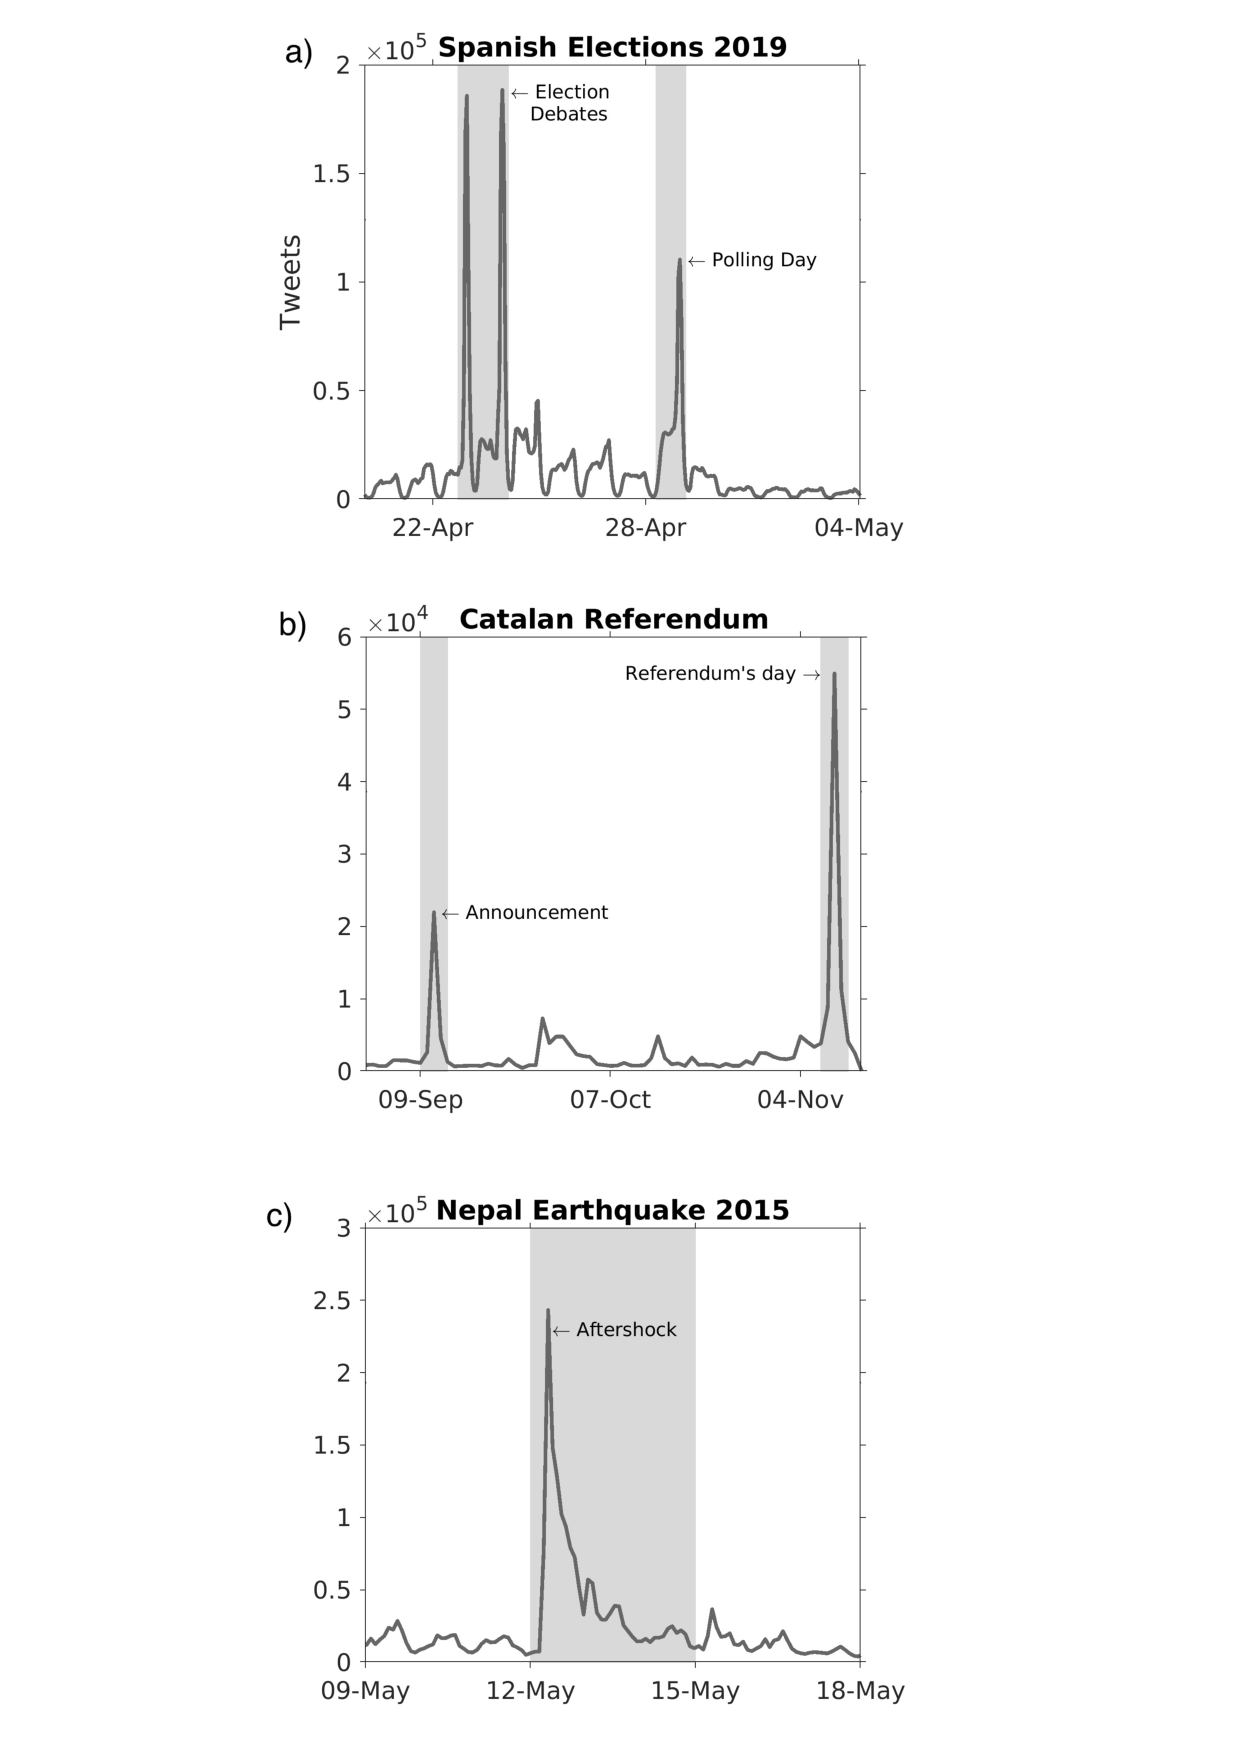
\includegraphics[width=1.05\textwidth]{figures/chp3/fig1new.pdf}

    \caption[Temporal evolution of the number of tweets]{Temporal evolution of the number of tweets for the considered datasets: the 2019 Spanish general elections (Panel a), the self-determination referendum in Catalonia in 2014 (Panel b), and the second major earthquake that hit Nepal in 2015 (Panel c). We highlight in gray the relevant events.
    }
   \label{chp3:fig:1}
\end{figure}

To capture the changes in attention, a methodology for extracting the topics being discussed during each interval must be developed, together with an intuition of competition and mutualism experienced by users in this techno-social context.  \\

\subsection{Information topics}
\label{chp3:1.2}

As the first step in deducing information topics from tweets, Figure~\ref{chp3:fig:1} shows the temporal evolution of the number of tweets for the datasets. All the datasets present clear high-activity periods related to external events, like the polling day for the Spanish elections (Figure~\ref{chp3:fig:1}a) or the referendum day for the Catalan Referendum (Figure~\ref{chp3:fig:1}b). These peaks in activity are surrounded by calmer periods characterized by much lower activity.  Since our aim is to study how competition for attention and users' interests vary between extraordinary and usual periods, we divide each dataset into different parts inspired by these different activities. More precisely,  for each dataset,  we determined the bulkiest spike in activity and set its duration as the size of the interval. In that way, we get intervals corresponding to ``peak'' and ``rest'' periods that are short enough to contain only a single event, along with having enough data during the calm periods. In the 2015 Nepal earthquake, the activity peak is $3$ day-long,  so we divided the dataset into intervals of precisely $3$ days. A similar reasoning was applied for the Catalan Referendum, where the extension of the largest spike is around $10$ days, and thus intervals are $10$ day-long. Yet,  since the Spanish elections dataset has a shorter duration, we set more irregular periods to guarantee enough tweets during the resting intervals.  \\

%This step is fundamental to measure the similarity between users and, eventually, quantifying the competition for attention that both users and memes experience over the development of the events.

Once we have defined the different periods, we focus on how to extract users' topics of interest from their tweets. To do so, we rely on a network theory approach developed precisely to infer information topics in Twitter \cite{weng2015topicality,cardoso2019topics,mussi2021topics}. It is based on hashtags co-occurrence, since users employ hashtags as keywords, to indicate the content of their message. Hashtags thus provide a straightforward representation of tweets' semantic context. If two or more hashtags appear in the same tweet, then it is safe to assume that there is a semantic association between them, as it usually happens to words frequently coinciding in texts \cite{turney2010words,martinez2011disentangling}. Based on this proxy,  we define information topics as cohesive clusters of hashtags that significantly appear together in tweets, capturing the commonalities in the hashtags' semantic context. From the perspective of the users, we assume that information topics will represent their set of interests. \\

The concrete methodology to determine topics is as follows: for each period considered in the data, if two hashtags appear in the same tweet, we connect them by a link, whose weight is proportional to the number of tweets where they co-occurred. To ensure that links only imply semantic associations between hashtags, we consider spurious and delete all the links whose weight is equal to or smaller than three. Once the weighted co-occurrence networks are built, we detect clusters of densely connected hashtags -- i.e. communities in the network science jargon-- and identify them as information topics. The communities in the different networks are detected using the OSLOM (Order Statistics Local Optimization Method) package \cite{lancichinetti2011oslom}, following the same procedure proposed in \cite{cardoso2019topics,mussi2021topics}. We choose OSLOM for community detection because it reveals overlapping communities, that is when nodes can belong simultaneously to more than one community. In this way, we guarantee that hashtags can have different meanings and hence be part of various topics. For example, four topics extracted from the Spanish elections dataset are depicted in Figure~\ref{chp3:fig:2} as wordclouds. They show  references to the most important dates, along with the names of several national parties. Some of these parties appear on more than one topic, indicating that they were present in several discussions. The combination of these words in each wordcloud makes clear that they represent different aspects of the discussion. For instance, the first wordcloud corresponds to election day and the third one revolves around the television electoral debate.\\
%Finally, extracting information topics for different periods will allows us to study how collective attention and the context of different memes evolves with the unfolding of the events.
\begin{figure}[t!]
    \centering
   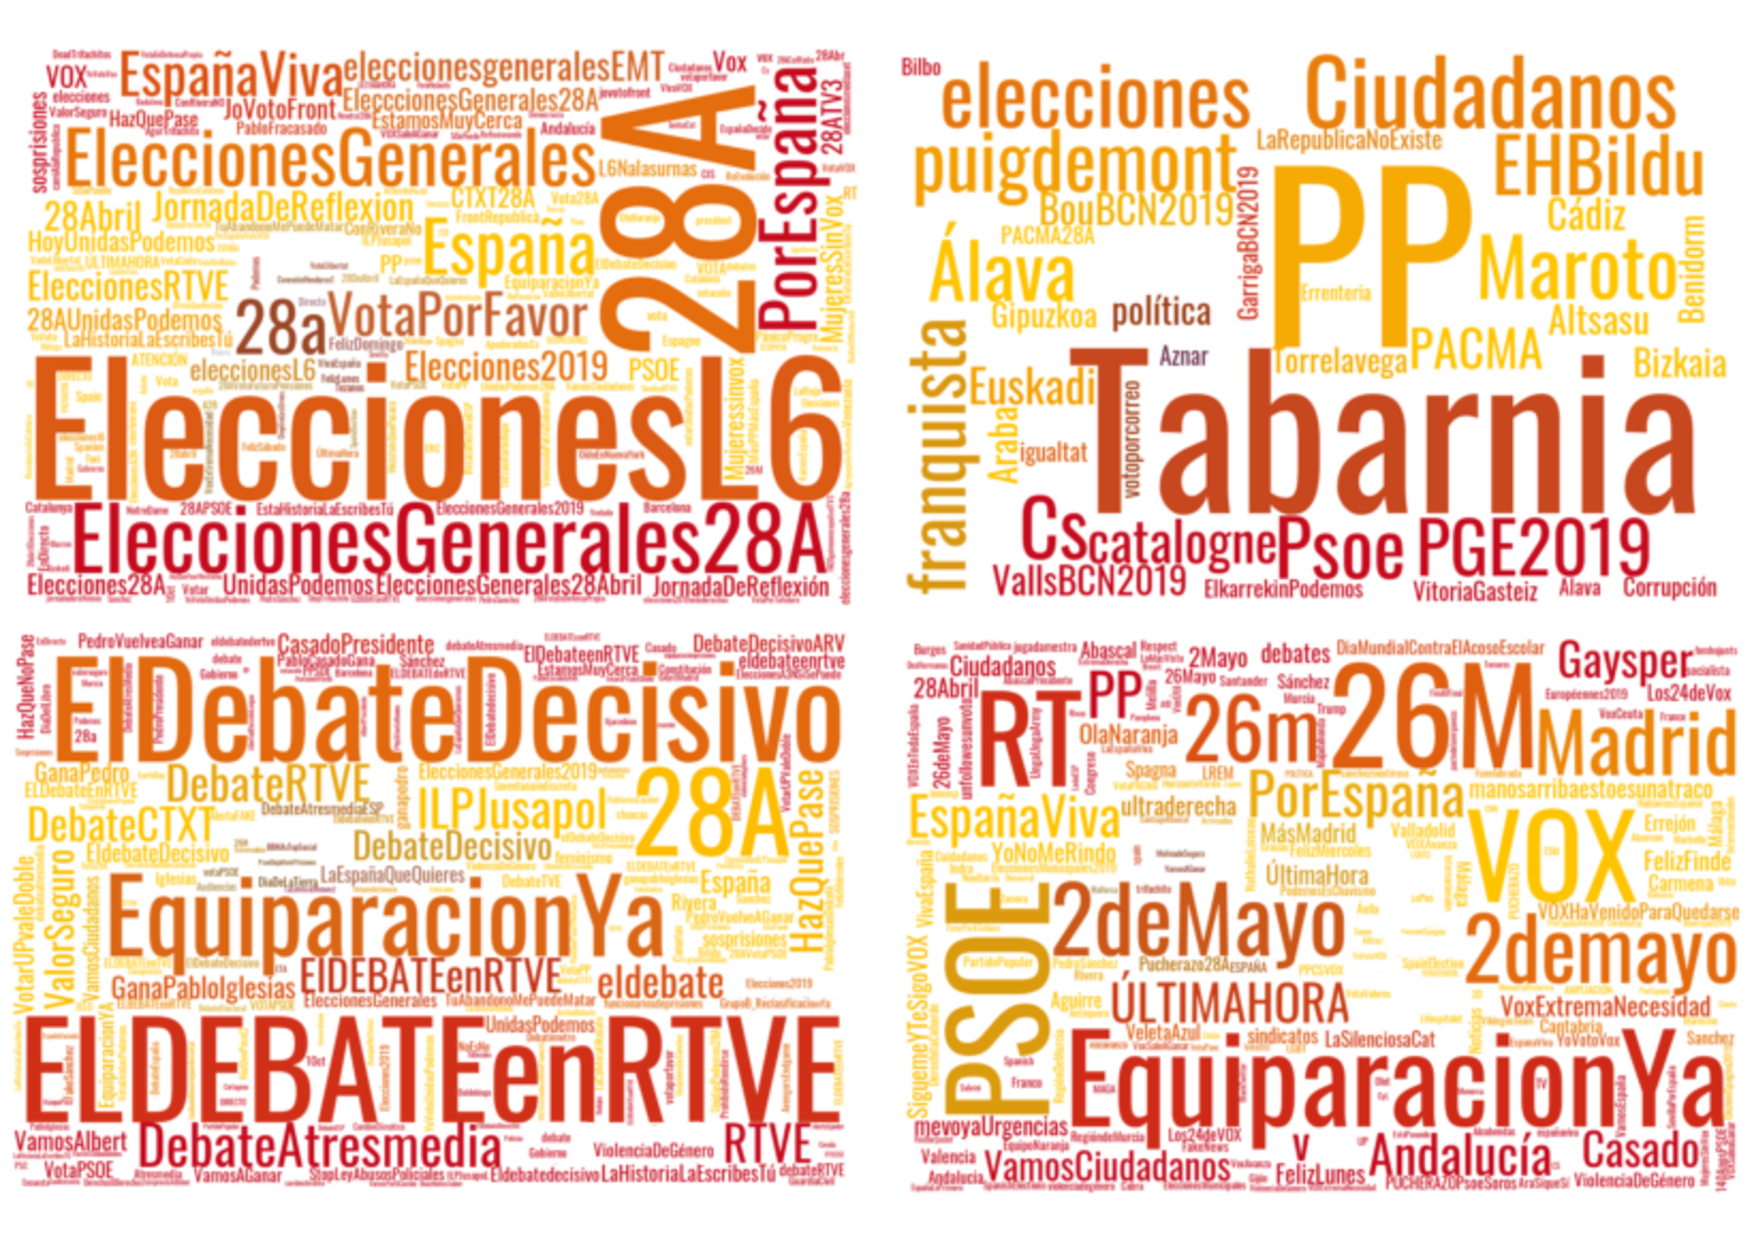
\includegraphics[width=1\textwidth]{figures/chp3/fig2.pdf}
   
    \caption[Word clouds of inferred topics]{Four example topics inferred from the Spanish general elections dataset. Each word cloud corresponds to one topic and it contains the most abundant hashtags, whose size is proportional to how many times they have been tweeted.}
   \label{chp3:fig:2}
\end{figure}

After obtaining the information topics from the data, we proceed to classify users into topics according to the hashtags they posted,
and ultimately,  to use the membership in various topics to detect users' interests. We proceed by building a feature vector $\mathbf{u}$ for each user, whose elements $u_i$ account for the number of occasions a hashtag belonging to topic $i$ was posted by the user. But since hashtags can belong to several topics within a period, the weight of each hashtag is split to take the number of communities they are part of into account. We assume one hashtag appearing only on one topic contributes to the corresponding entry of $\mathbf{u}$ by adding one. Conversely, a hashtag that is part of two topics $i$ and $j$  contributes $0.5$ to each $u_i$ and $u_j$. Finally, the value of $u_i$ is considered to be equivalent to the user's interest in topic $i$. The same method can be applied to build a counterpart hashtag vector $\mathbf{h}$ that quantifies their share of different topics.  In the diagrams of Figures~\ref{chp3:fig:3}a and \ref{chp3:fig:3}b we show a toy example of how vectors $\mathbf{u}$ and $\mathbf{h}$ are built. There, the hashtags posted by a user happen to be classified into three topics. One hashtag (\textit{\#lorem)} appears in topics $1$ and $2$ and therefore only adds $0.5$ to the corresponding entries $u_1$ and $u_2$. Likewise, its hashtag vector has a $1$ in the entries that correspond to topics $1$ and $2$. \\
 
A user vector quantifies how attention is scattered across different topics and how external events spotlight specific issues. In this sense, if information topics are thought of as ecological niches \cite{williams2000niche}, then $\mathbf{u}$ is the empirical equivalent of the niche profile proposed in \cite{cai2021niches,palazzi2021ecological} and introduced in Section~\ref{chp:methods:niche}. To build more intuition about this, let's define the ecological niche as ``the range of environmental conditions in which a population can persist'' \cite{hutchinson1957concluding}. Moreover, the niche profile of a species is formulated as the precise distribution of conditions in which that species thrives  \cite{williams2000niche}. For example, in Figure~\ref{chp3:fig:3}b, the user will prosper more in topic $3$ than in topic $1$. For cross-guild species (e.g., pollinators and plants), the niche proximity catches the complementarity of possible mutualistic partners. On the other side, within a guild, species with similar niches tend to share the same necessities (e.g., for nesting sites and light requirements). In that situation, the niche overlap instead captures competition for resources between species.\\

Returning to online social systems, information topics can be thought of as the environmental conditions in which users and hashtags thrive. individual interests may trigger competition too, and in this case, for attention. Users rival their peers for getting their posts read. In the same way, if an external event has focused attention on a specific theme, the hashtags related to it will suffer stronger competition for being chosen to appear on the users' screens. Lastly, users, aiming to reach potentially larger audiences, choose between hashtags when posting about popular content, leading to a kind of mutualistic interaction. Returning to our example, the user will benefit from posting hashtag \textit{\#lorem} again because it is very aligned with their interests, but posting a hashtag belonging to a hypothetical $4$\textit{th} topic would be zero since it is out of their scope. \\
\begin{figure}
   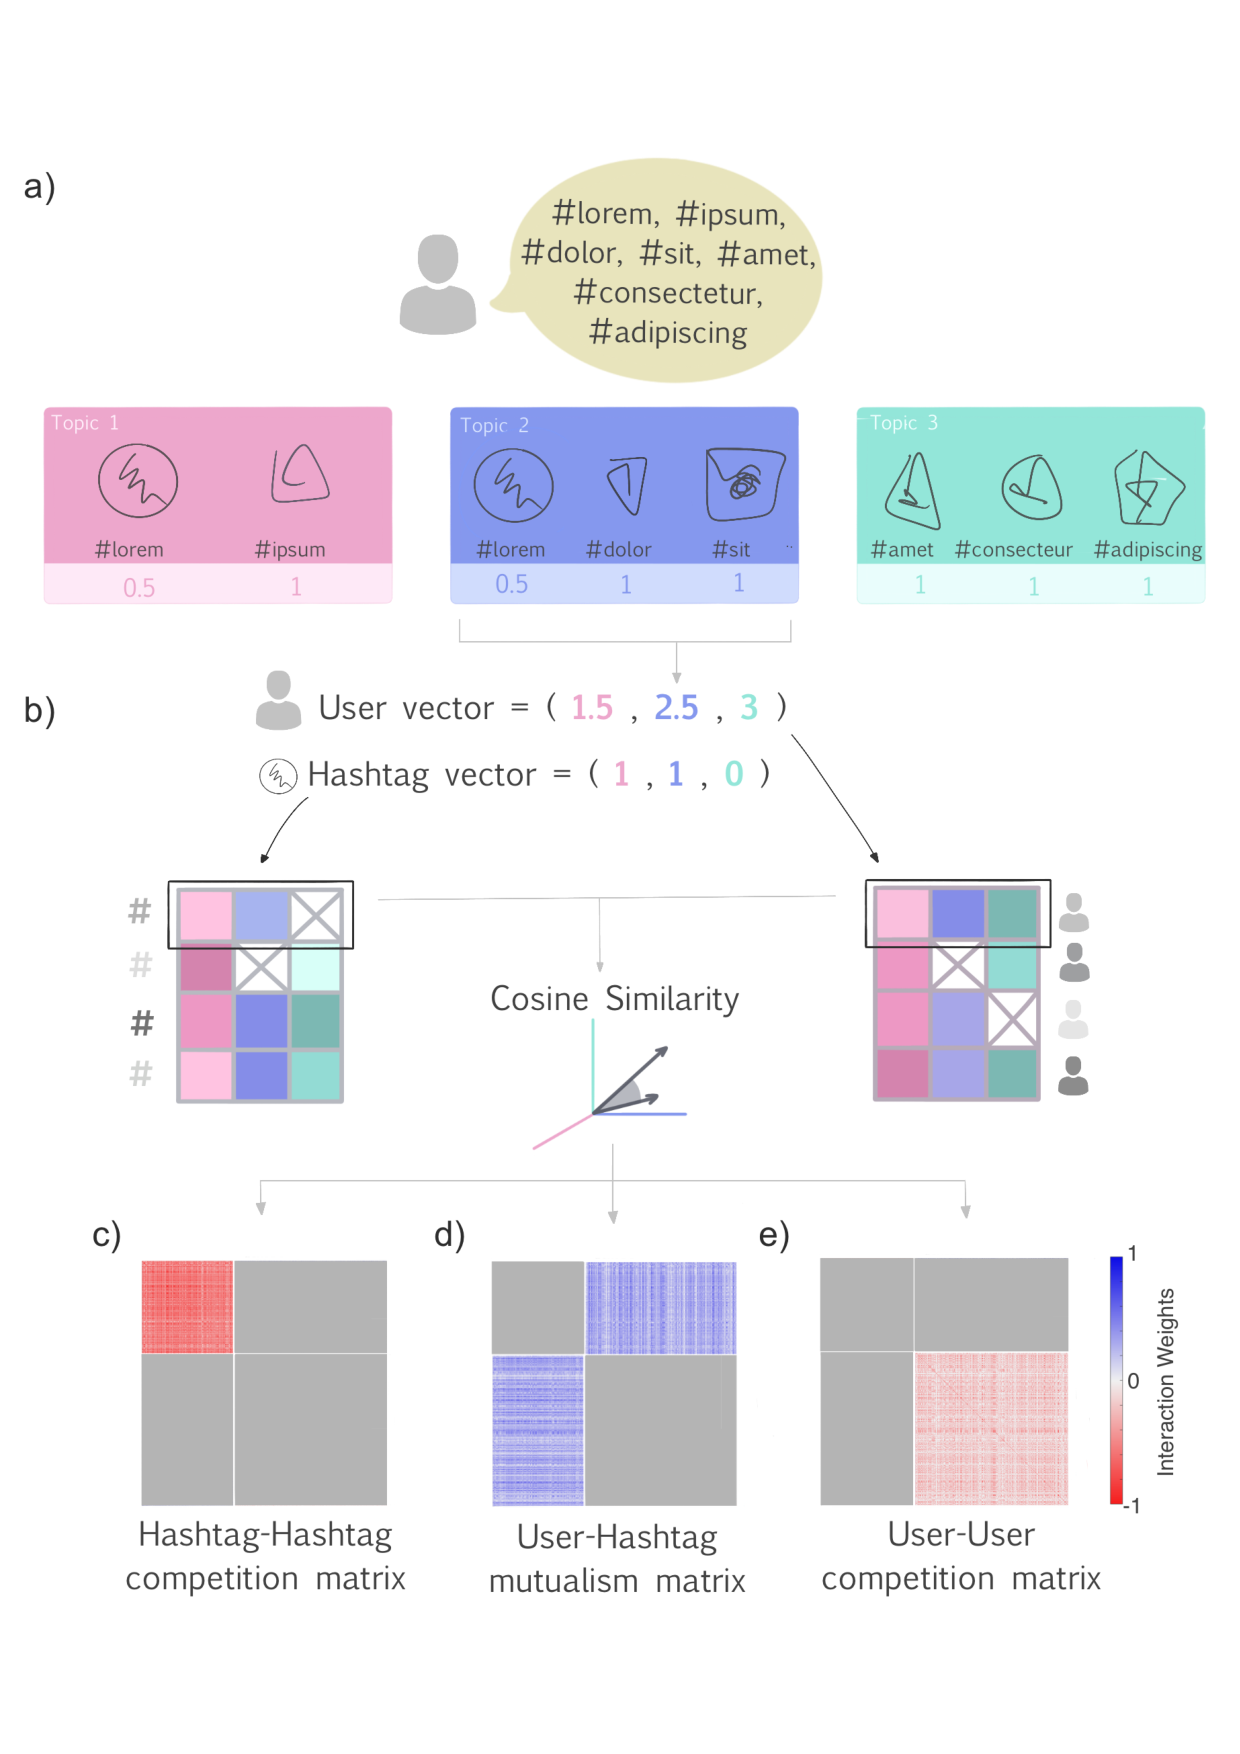
\includegraphics[width=0.95\textwidth]{figures/chp3/fig3.pdf}
    \centering
   
    \caption[Methodology for extracting user-topic and hashtag-topic vectors]{Illustration of the methodology for extracting user-topic and hashtag-topic vectors, and ultimately creating the competitive and mutualistic matrices. (Panel a) Using the algorithm proposed in \cite{cardoso2019topics}, hashtags are classified into topics. (Panel b) Hashtag-topic vectors encode the membership of each hashtag to one or more topics, so their dimension is the number of topics obtained. When a hashtag is part of more than one topic its weight is evenly divided between all the topics it belongs to. User-topic vectors are calculated from the hashtags tweeted by each user.  (Panels c, d, and e) The cosine similarity of each pair of user and hashtag vectors is tantamount to topic overlap. (Panels c and e) The elements of the hashtag-hashtag (user-user) competition matrices are computed proportionally to the topic similarity between hashtags (users). (Panel d) Similarly, the mutualism matrix is built as the similarity between hashtags and users. }
   \label{chp3:fig:3}
\end{figure}

To quantify the amount of competition users endure every period in the datasets, we calculate how similar $\mathbf{u}$ vectors are between users. For each pair of user vectors $\mathbf{u}$ and $\mathbf{v}$ we measure, inspired by the concept of niche overlap, their cosine  similarity: 

\begin{equation}
    sim_{cos}(u,v) = \frac{\mathbf{u} \cdot \mathbf{v}}{\left\Vert \mathbf{u} \right\Vert  \left\Vert  \mathbf{v} \right\Vert}.
\label{eqsim}
\end{equation}

In this way, we define a measure that goes from $0$ (where users have totally disconnected interests) to $1$ (perfectly aligned users). On the other side, hashtag competition can also be calculated likewise, using hashtag vectors $\mathbf{h}$ instead of $\mathbf{u}$ (see Section~\ref{chp3:1.4} for more details).  \\

Ultimately, to quantify how much mutualism a pair of a user $\mathbf{u}$ and hashtag $\mathbf{h}$ experiences, we also measure the cosine similarity:

\begin{equation}
    sim_{cos}(u,h) = \frac{\mathbf{u} \cdot \mathbf{h}}{\left\Vert \mathbf{u} \right\Vert  \left\Vert  \mathbf{h} \right\Vert}.
\end{equation}

We obtain, like for competition, $0$ similarity for pairs of users and hashtags without any topic in common, and a maximum of $1$ for totally aligned pairs.

\subsection{Dynamical model of users' attention}
\label{chp3:1.3}
Once developed a method to classify users and hashtags according to their interests, we can  use their similarities to measure how much competition and mutualism is experienced by each agent. Furthermore, to get an additional understanding of the driving mechanism behind changes in collective attention, we also utilize an ecology-inspired visibility optimization model \cite{palazzi2021ecological}, proposed to explain the structural shifts in the user-hashtag interaction networks through an event. \\

Following the analogies between information ecosystems \cite{palazzi2021ecological,plata2021neutral} and ecological communities, the model is based on an adaptive niche model \cite{cai2021niches}. Its main assumption is that the relations among species adaptively change to maximize the abundance of single species \cite{suweis2013emergence}. For information ecosystems, an optimization process where users seek to maximize their visibility is supposed to drive the attention dynamics. Hashtags and users are interpreted as species of a mutualistic community from two separate guilds --e.g., pollinators and plants in natural ecosystems. Competitive interactions occur between within-guild species (between hashtag-hashtag and user-user pairs), while mutualism takes place between species of different guilds (user-hashtag). Species dynamics follows Lotka-Volterra equations with a Holling-Type II functional response (see Section~\ref{chp:methods:LV}): 

\begin{equation}
\label{eq:dyn}
{\begin{aligned}{\frac {dn_i^U}{dt}}&=n_i^U \left(\rho_i^U - \sum_j \beta_{ij}^{UU}n_j^U + \frac{\sum_k \gamma_{ik}^{UH}n_k^H }{1+ h \sum_l \theta_{il}n_l^H} \right), \\[6pt]
{\frac {dn_k^H}{dt}}&=n_k^H \left(\rho_k^H - \sum_l \beta_{kl}^{HH}n_l^H + \frac{\sum_i \gamma_{ki}^{HU}n_i^U }{1+ h \sum_j \theta_{kj}n_j^U} \right).
\end{aligned}}
\end{equation}
where $n_i^U$ and $n_k^H$ represent the abundance (visibility) of species belonging to the users' ($U$)  or hashtags' ($H$) guild, $\rho_i^U$ and $\rho_k^H$ stand for their respective growth rates, while  $h$ is the handling time of the Holling-Type II mutualistic functional response. Matrices $\boldsymbol{\beta^{UU}}$, $\boldsymbol{\beta^{HH}}$ and $\boldsymbol{\gamma^{UH}}$ encode the strength of users' and hashtags' competitive and mutualistic interactions, respectively. Finally, $\boldsymbol{\theta}$ is the adjacency matrix of the bipartite network. An element $\theta_{ik}^{UH}$ equals one whenever user $i$ is employing hashtag $k$ in their posts. \\

The optimization process works as proposed in \cite{suweis2013emergence}, where users change their mutualistic connections to randomly selected hashtags, and the new rewiring is kept if and only if it induces an increase in abundance (a.k.a. visibility). Otherwise, the initial link is re-established (check Figure~\ref{fig:nicheModel}). At fixed time intervals, we randomly choose a user $i$, and rewire one of its current connections to a new random hashtag $l$. The link to rewire is selected with a probability $p_{il} \propto 1 - 1/k^{H}_{l}$ where $k^{H}_{l}$ is the  number of users connecting with hashtag $l$. This ensures that every hashtag has at least one mutualistic interaction. After the rewiring, we let the system evolve until it reaches a new equilibrium. If at this point the user $i$'s abundance is larger than before the rewiring, the new link is kept; otherwise, we restored the previous configuration.   \\

It should be noted that, in our model, only users are the active agents in the optimization process since they choose what hashtags to tweet to maximize their abundance (the proxy for visibility). Therefore, the changes in hashtags' connections are solely due to users' actions.  \\

\subsection{Estimating competition and mutualism from data}
\label{chp3:1.4}
Finally, we estimate the matrices of interaction strength among species ($\boldsymbol{\beta^{UU}}$, $\boldsymbol{\beta^{HH}}$ and $\boldsymbol{\gamma^{UH}}$) from our data following the approach proposed by Williams and Martinez \cite{williams2000niche}. 
Mutualistic and competitive strengths are proportional to niche overlap between species of the opposite (mutualism) and the same (competition) guilds. As introduced in Section~\ref{chp3:1.2}, the niche overlap $G_{ij}^{gg'}$ between species $i$ from guild $g$ and species $j$ from guild $g'$ is estimated as the cosine similarity between the topic vectors of $i$ and $j$. For the competition, the elements of the matrices $\beta_{ij}^{HH}$ and $\beta_{kl}^{UU}$ are simply proportional to the niche overlap by a global factor $\Omega_c$ that tunes the absolute interaction strength: $\beta_{kl}^{HH} \propto \Omega_c \cdot G_{kl}^{HH}$ and $\beta_{ij}^{UU} \propto \Omega_c \cdot G_{ij}^{UU}$. Correspondingly, the elements of the mutualistic matrix are defined as  $\gamma_{ik}^{UH} \propto \Omega_m \cdot G_{ik}^{UH}$. For the particular case of mutualism, the interaction strength matrix $\gamma_{ik}^{UH}$ is multiplied by $\theta_{ik}$ to incorporate the fact that user $i$ may not ($\theta_{ik}=0$) or may ($\theta_{ik}=1$) interact with hashtag $k$. Lastly, to compare the two strengths, and without losing generality, we set $\Omega_c = \Omega_m$. 


\section{The rise and fall of buzz: visibility optimization drivers collective attention}
\label{chp3:2}

Our analyses start by splitting our three datasets into different periods based on their activity (i.e., the total number of tweets produced), and following the approach explained in Section~\ref{chp3:1.2}. The objective of this division is to distinguish what we define as peak periods from resting periods. Peak periods are exogenous events that produce large activity on Twitter, such as the referendum day for the Catalan dataset or the TV debate for the Spanish elections. On the other side, during rest periods, the discussion is still happening but not driven by major external events. We will use the calmer periods to set a baseline for activity and collective attention and to contrast them with peak periods.  \\

\begin{figure}[t]
   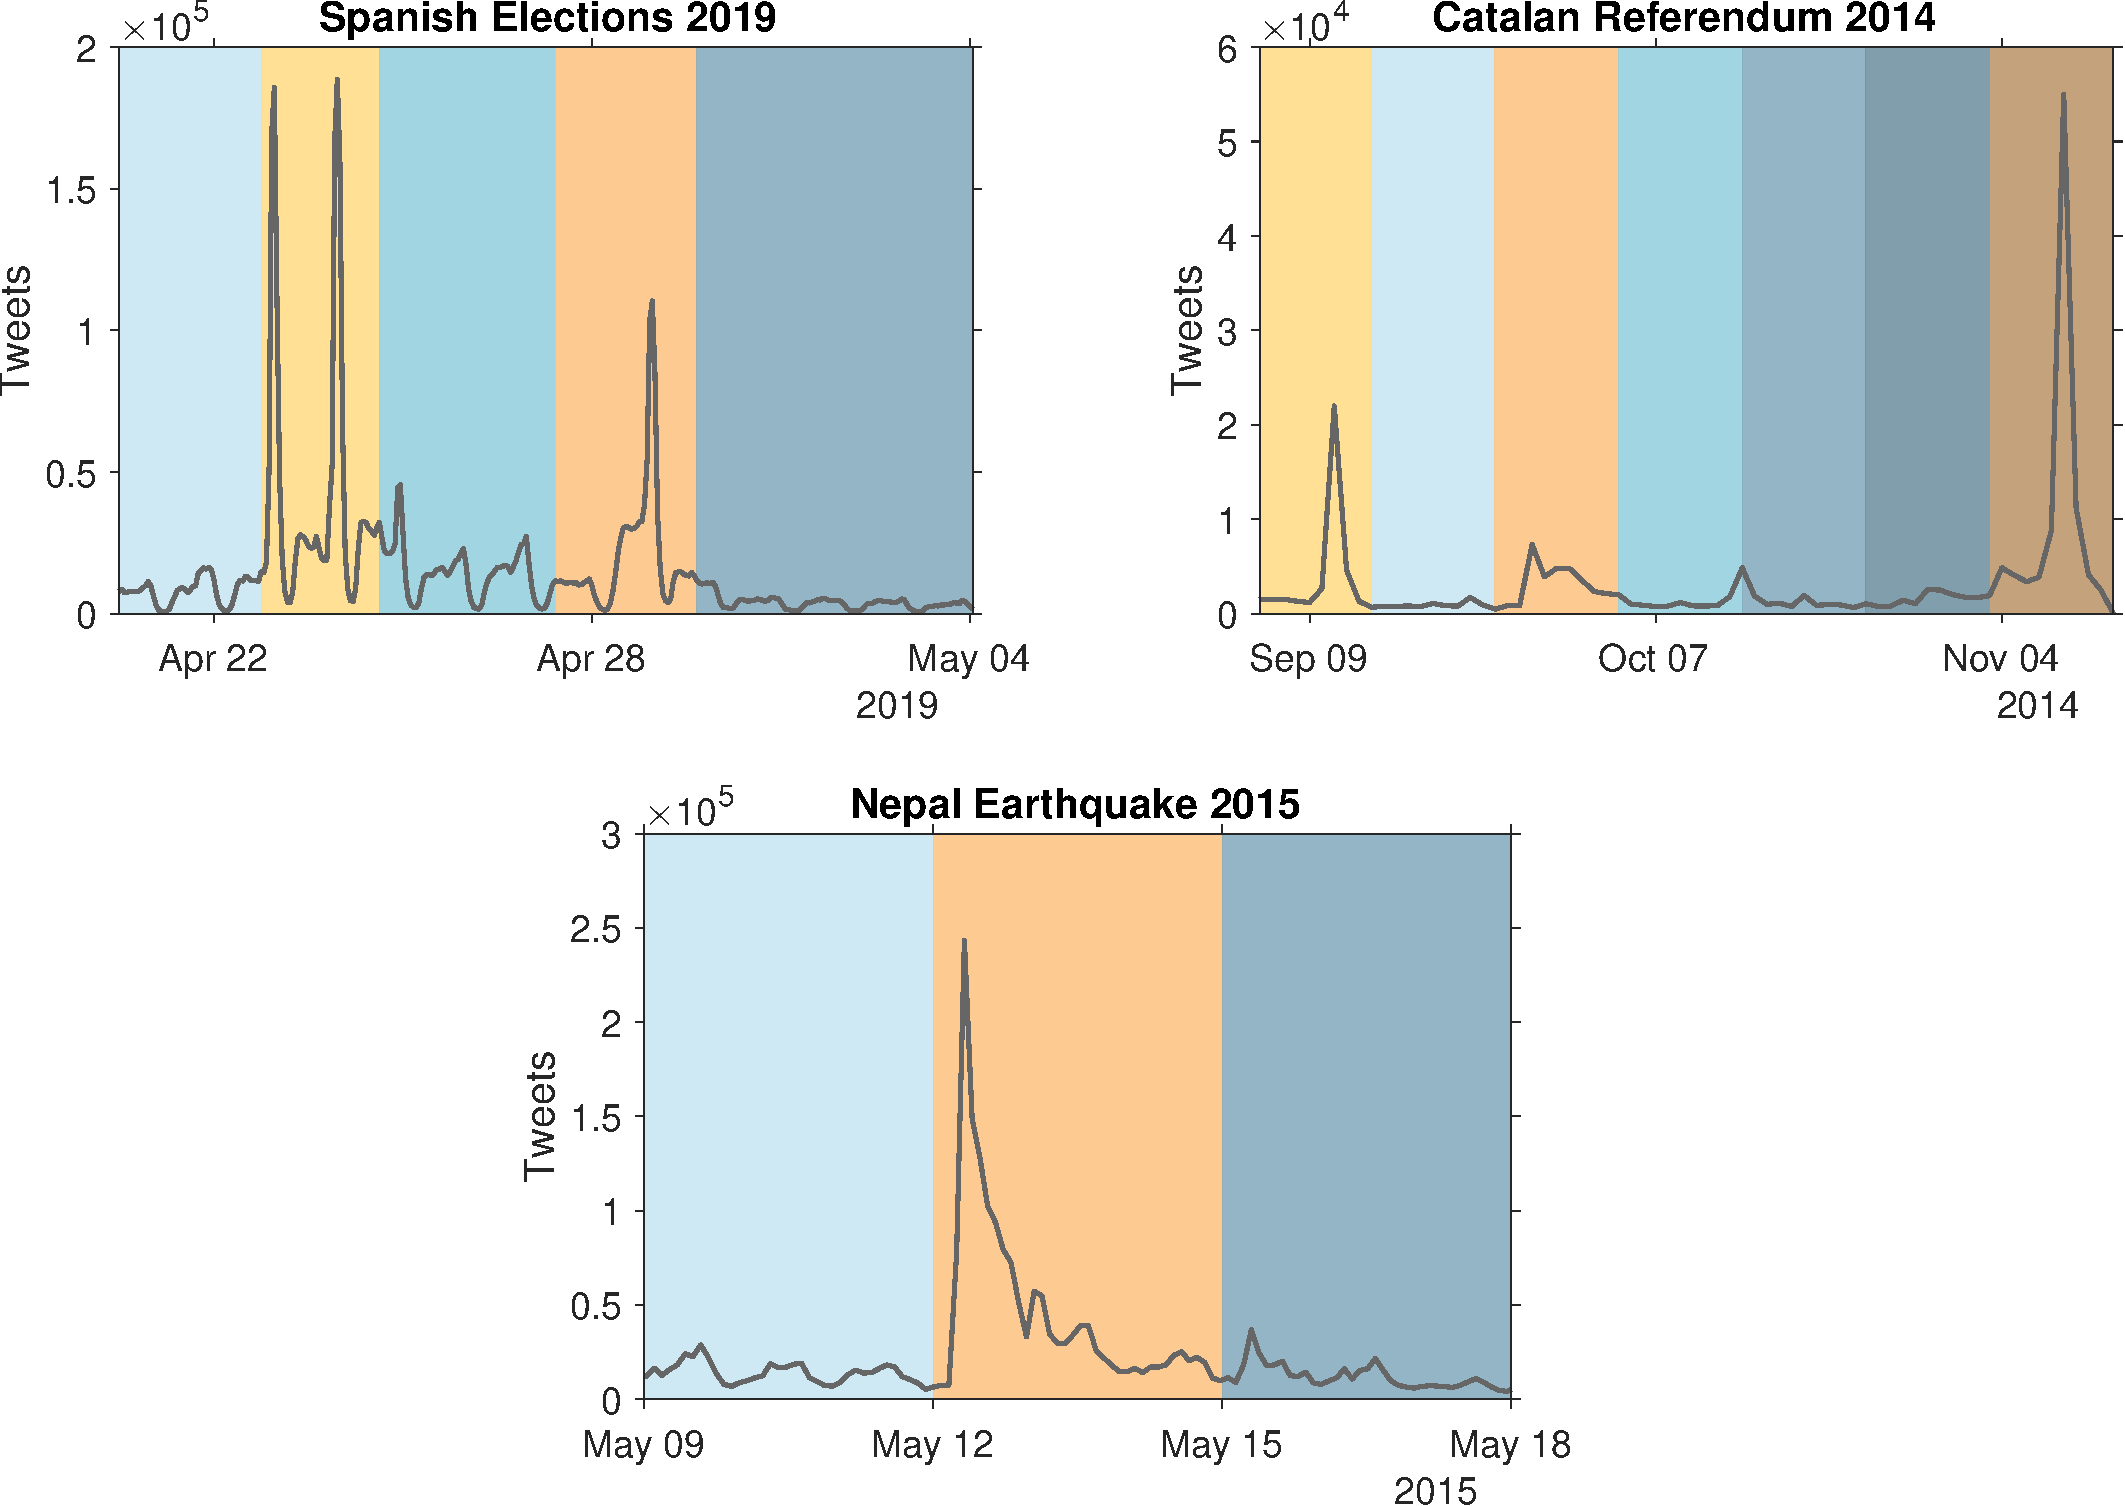
\includegraphics[width=1\textwidth]{figures/chp3/fig4a.pdf}
   
    \caption[Time evolution of the number of tweets by activity periods]{(Panels a-c) Time evolution of the number of tweets in the different datasets divided by activity periods. The colors of each period are just for visualization purposes.}
   \label{chp3:fig:4a}
\end{figure}

\begin{figure}
   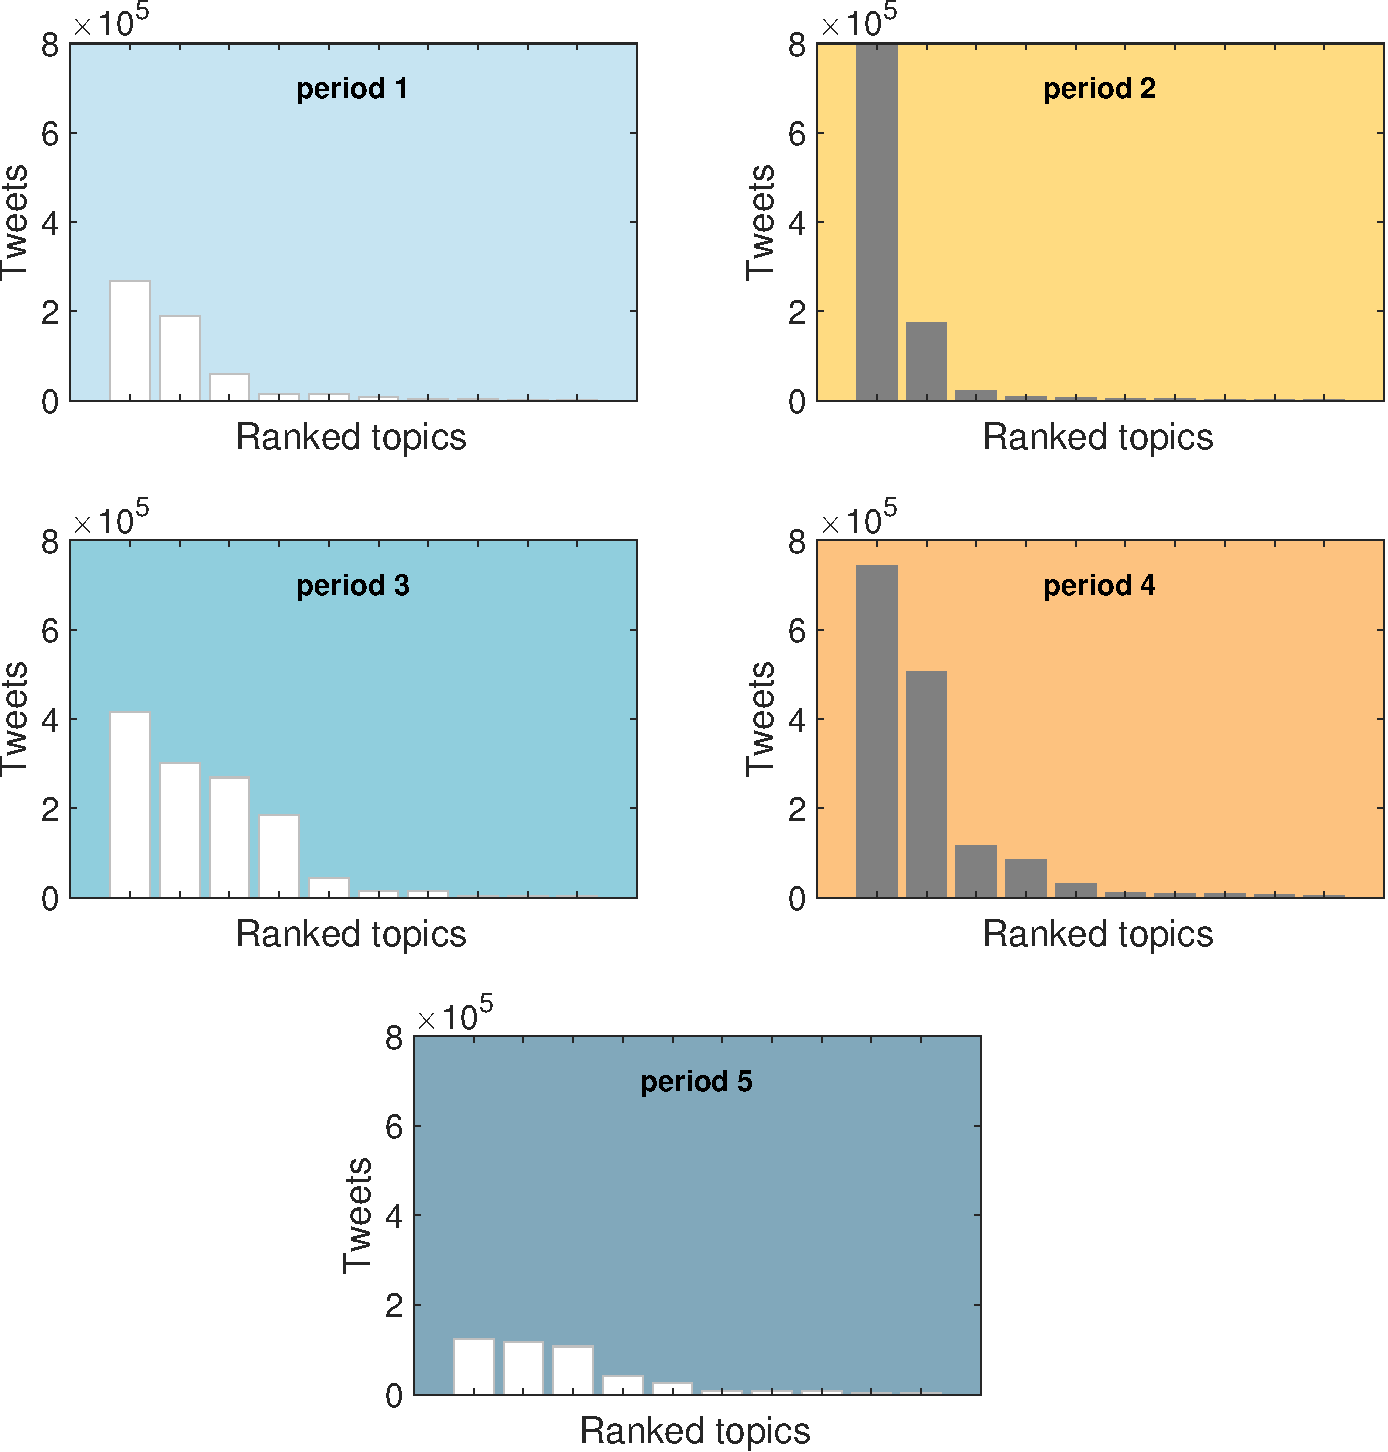
\includegraphics[width=1\textwidth]{figures/chp3/fig4b.pdf}
   
    \caption[Activity distribution through topics and periods]{(Activity (number of tweets) in the largest $10$ topics for every period of the Spanish elections dataset. Gray bars mark the peak periods.}
   \label{chp3:fig:4b}
\end{figure}
Figures~\ref{chp3:fig:4a}a-c illustrate the divisions of our datasets. For the 2109 Spanish elections dataset (Figure~\ref{chp3:fig:4a}a) we identify $5$ periods, where the second and fourth cover the main large events, while the fifth represents our baseline of activity. The third period is a combination of high activity and calmer times since it has smaller events taking place. In the 2104 Catalan referendum dataset (Figure~\ref{chp3:fig:4a}b), we identify $7$  different periods: the second, fourth, fifth, and sixth as resting states; and the first, third, and seventh as peaks. Finally, in the 2015 Nepal earthquake dataset (Figure~\ref{chp3:fig:4a}c), we define just three periods, with the first one representing the baseline state, the second period being the peak, and the third one a mixture of peak and rest.  \\

\subsection{Topics evolution}\label{chp:3:topicsevol}
\label{chp3:2.1}
Once specified our active and baseline intervals, we extract the topics of every period to study how the hashtag networks and users' interests evolve through time. Following the procedure described in  Section~\ref{chp3:1.2}, we create a hashtag co-occurrence network for each period and get the most important communities from it, which define our topics. \\

From the hashtag co-occurrence networks, we can study how topics evolve period by period, and how external events reorganize the corresponding discussions. Table~\ref{tab:nets}  summarizes the main features of the networks extracted from each considered dataset. A result that stands out is that although networks of different periods have different sizes, the number of topics (i.e. communities in the networks) is almost constant.  For example, the number of hashtags (i.e. nodes) in the Spanish elections dataset increases a $44\%$ between the most and least active periods --it varies from $1313$ to $1899$--  but the number of topics in each period only goes up by a $28\%$ --it ranges from $77$ to $60$. This fact deviates from our hypothesis that collective attention focuses on one or not many ``main topics'' during external events. However, considering not only the number of topics but also their activity, this discrepancy is solved. In Figure~\ref{chp3:fig:4b}, for the Spanish elections dataset, we show how activity --in terms of the number of tweets the topics generate-- distributes among the $10$ largest topics for the different periods. We can observe that activity, in general, is highly heterogeneous. However, during high-activity periods (plots with gray bars), this tendency intensifies with one or two topics gathering almost the $90\%$ of the tweets together. We get similar results for the other datasets, not shown in Figure~\ref{chp3:fig:4b}.  \\

\begin{table}
    \centering
\caption[Summary of the co-occurrence networks obtained from each dataset]{\label{tab:nets} Summary of the co-occurrence networks obtained from each dataset.}
\footnotesize
\begin{tabular}{c c c c c c }
\hline
Dataset & Period & No. hashtags & No. links & No. topics\\
\hline \hline
%Spanish & & & &\\
Spa. Elec. & 1 & 1344 & 6866 & 75 \\
& 2 & 1714 & 11587 & 68 \\
& 3 & 1899 & 12026 & 77\\
& 4 & 1736 & 12373 & 63\\
& 5 & 1313 & 5114 & 60\\

\hline

%Catalan Ref & & & &\\
Cat. Ref. & 1 & 703 & 3170 & 9 \\
& 2 & 310 & 863 & 20 \\
& 3 & 586 & 2070 & 10\\
& 4 & 350 & 1037 & 21\\
& 5 & 338 & 911 & 16\\
& 6 & 362 & 1112 & 13\\
& 7 & 1602 & 5837 & 12\\

\hline
%Nepal & & & &\\
Nepal & 1 & 471 & 1564 & 29 \\
& 2 & 771 & 4739 & 27 \\
& 3 & 670 & 2921 & 33\\

\hline

\end{tabular}\\
\end{table}


\begin{figure}[t]

    \centering
   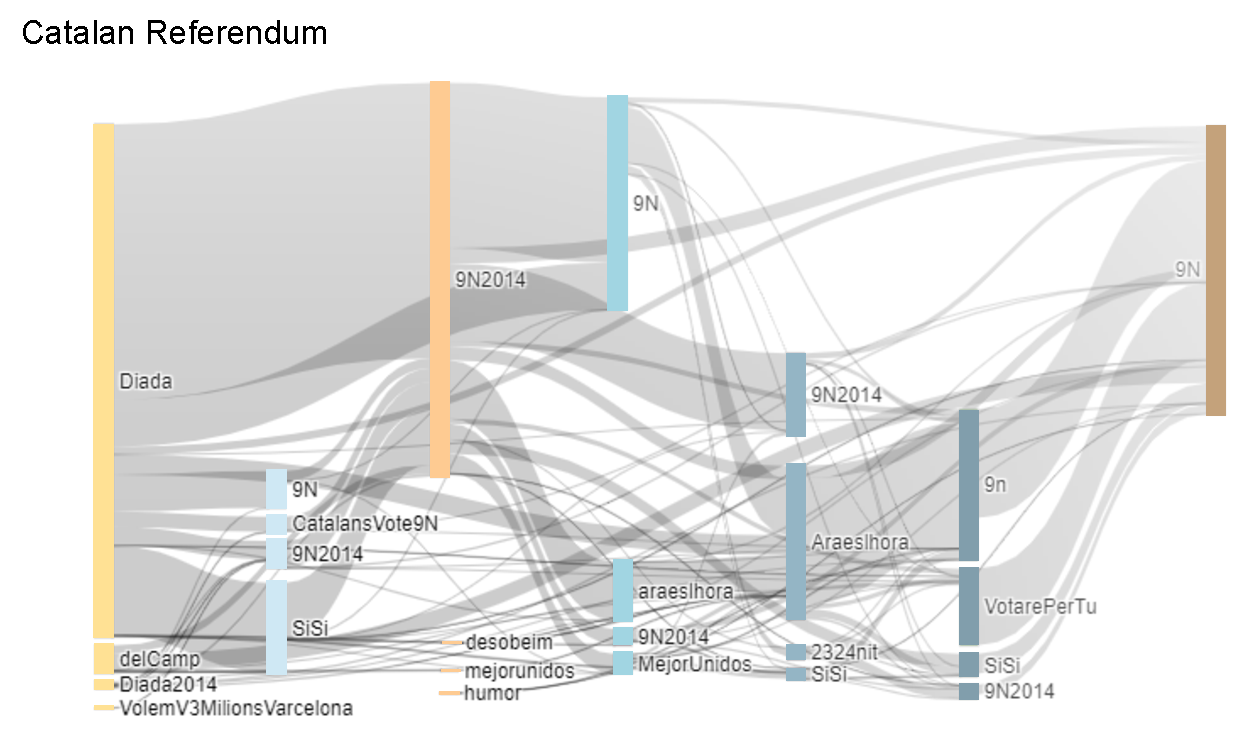
\includegraphics[width=1.05\textwidth]{figures/chp3/fig5.pdf}
   
    \caption[Alluvial diagram of topic sizes]{Topics' development for the Catalan referendum dataset is illustrated with an alluvial diagram. Boxes represent topics (communities in the co-occurrence network). Their colors encode the different periods, and their sizes are proportional to the number of tweets that belong to each topic. To ensure readability visibility, only the four largest topics are shown for each period. Flows represent the volume of tweets moving from one topic in a certain period to another topic in successive periods.}
   \label{chp3:fig:5}
\end{figure}

\begin{figure}[t]
    \centering
   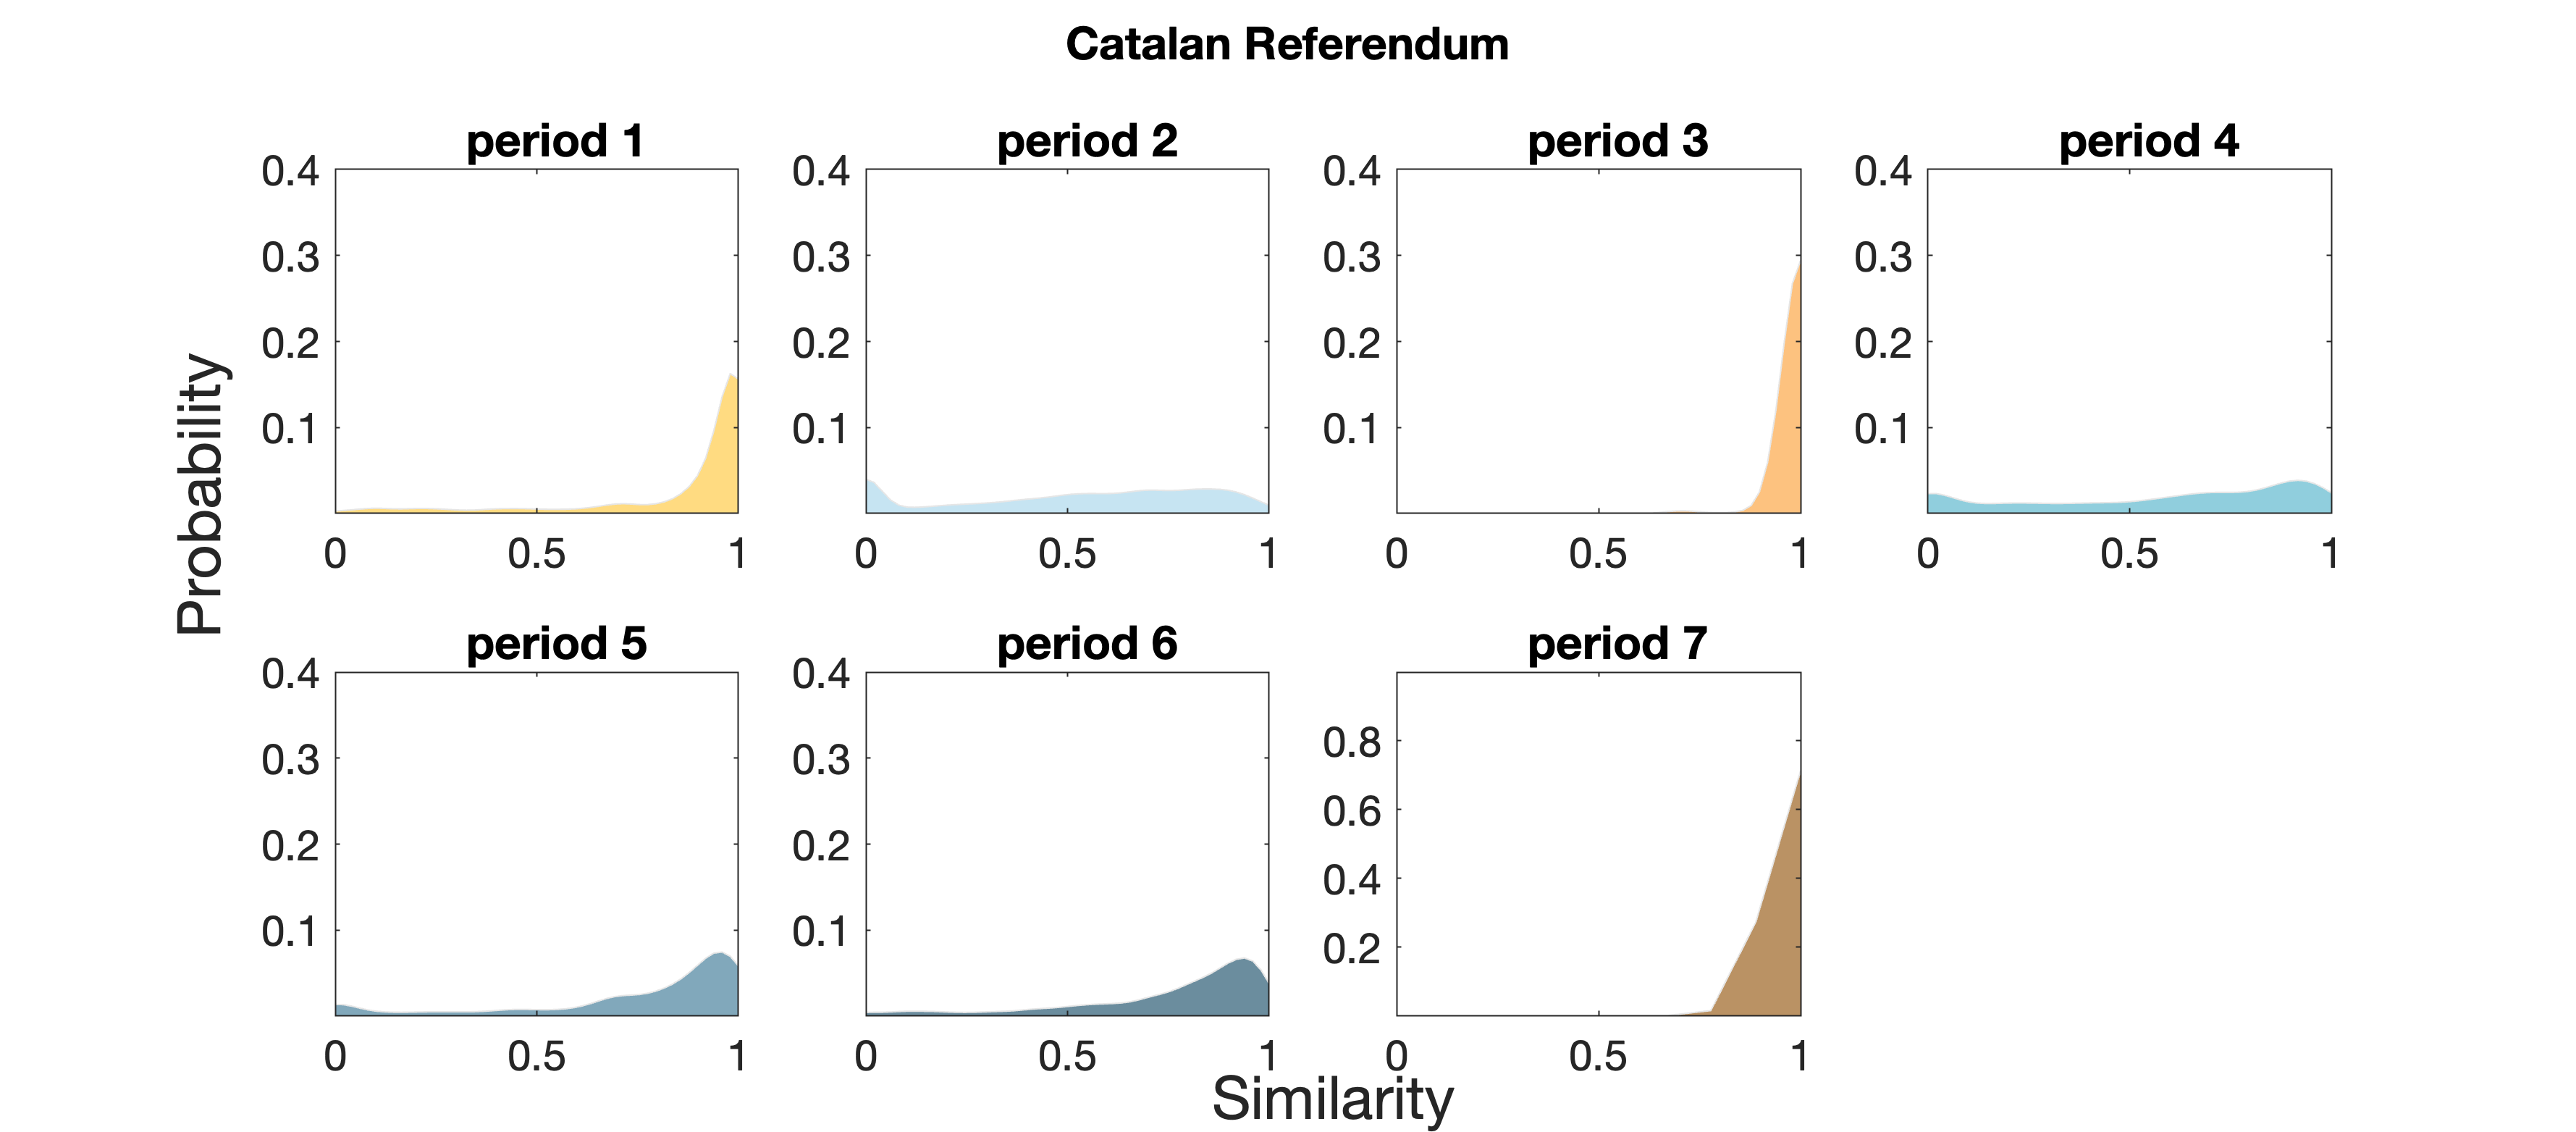
\includegraphics[width=1.05\textwidth]{figures/chp3/similarity_catalonia_nolog.png}
   
    \caption[Cosine similarity distribution of user-topic vectors]{Cosine similarity distribution of user-topic vectors for the most active users of the Catalan referendum dataset. The cosine similarity has been calculated following Eq.~\ref{eqsim}. The most active users are the ones that have taken part in the discussion for at least $90\%$ of the time and posted a minimum of $10$ tweets within the whole period, which comprise around $400$ accounts. Shaded areas denote peak periods.}
   \label{chp3:fig:6}
\end{figure}

These last two results --the heterogeneous distribution of activity during peak events shown in Figure~\ref{chp3:fig:4b}, and the consistent number of topics over the periods,  as detailed in Table~\ref{tab:nets}--, define a precise scenario. During periods of ordinary activity, users focus on their own interests, and hashtags compete for attention inside the specific discussions. When collective attention is captured by an external event, initial topics stay active but generate less activity. To visualize how attention shifts from the different topics over time, we have created an alluvial diagram for the activity around the topics through periods. Figure~\ref{chp3:fig:5} shows the diagram for the Catalan referendum dataset (we have obtained equivalent results for the other datasets, not shown). The size of each block is proportional to the number of tweets, and only the flows of activity of the four bulkiest topics are considered. During peak periods (first, third, and seventh), the flows merge into one single topic (``Diada'', ``9N2014'' and ``9N'', respectively). When external events dissipate, flows break apart into different discussions again, and some hashtags are not posted during calm intervals, but recover popularity during high-activity periods. This behavior can see seen, for example, by looking at the extensive flows moving right from the first period to the third one.


\subsection{Users' similarity}
\label{chp3:2.2}

Having previously investigated how extraordinary events influence hashtags' use and activity, we can now concentrate on the opposite side of the equation: user behavior. We measure the overlap in interests between user pairs with the cosine similarity of user-topic vectors. A higher average similarity will indicate that people are paying more attention to a smaller number of topics, which will lead to more competition. \\

Figure~\ref{chp3:fig:6} shows the distribution of similarity between all potential pairs of the $400$ most active users from the Catalan referendum dataset (active users for at least $90\%$ of the time and posting at least $10$ tweets containing hashtags).  The outcomes  match what we discovered for the hashtags, as expected. Users' similarity is homogeneously distributed between $0$ and $1$ during periods of low activity (i.e., second and fourth periods), indicating that independent discussions with nearly equivalent activity are occurring. On the other hand, high activity periods are marked by a nearly perfect alignment of users, with the similarity distribution peaking at exactly one: everyone is chatting about the same issue.

\begin{figure}[t]
    \centering
   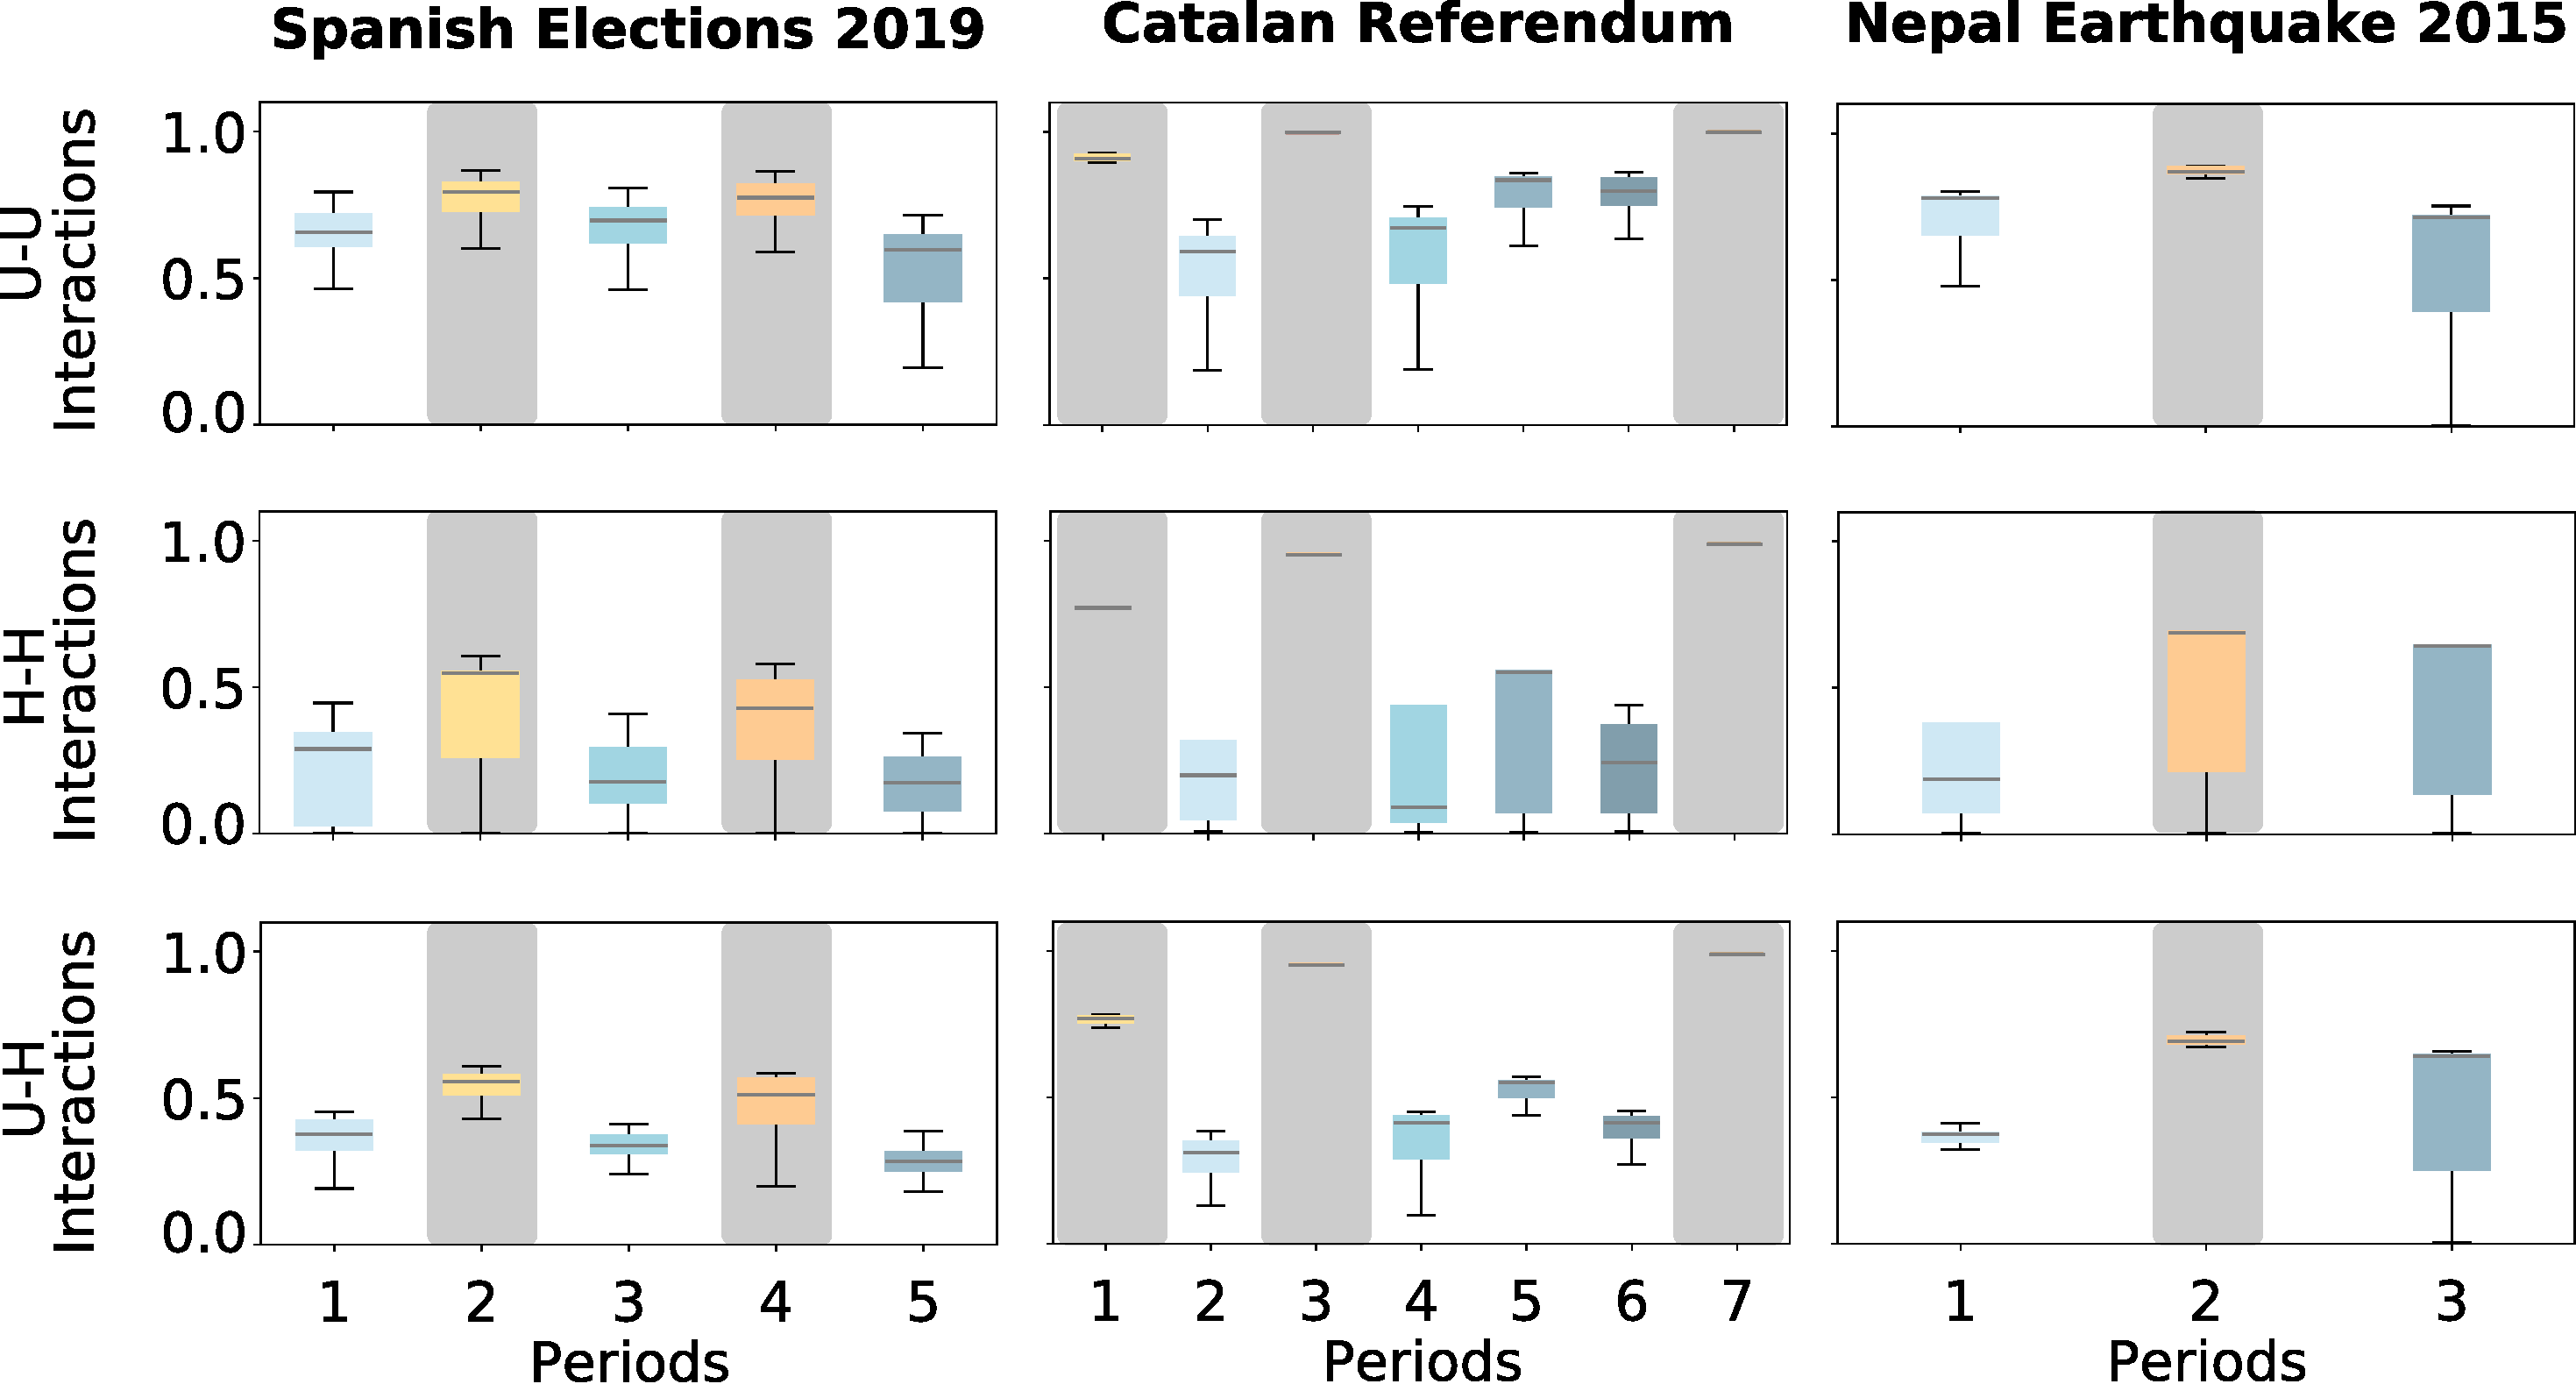
\includegraphics[width=1\textwidth]{figures/chp3/fig7.pdf}
   
    \caption[Strength estimations for competitive and mutualistic interactions]{Strength estimations for hashtag-hashtag and user-user competitive interactions (first and second row), and user-hashtag mutualism (third row) for the $400$ most active users and the hashtags they wrote. The interaction strength is the average value of the elements of the matrices $\beta^{HH}$, $\beta^{UU}$, and $\gamma^{UH}$. The gray horizontal line in the box plots is the median of the distribution, and the colored boxes have a length corresponding to the 25th-75th percentiles. As usual, shaded areas mark peak periods.}
   \label{chp3:fig:7}
\end{figure}



\subsection{Quantifying competition and mutualism during exceptional events}
\label{chp3:2.3}


\begin{figure}
    \centering
   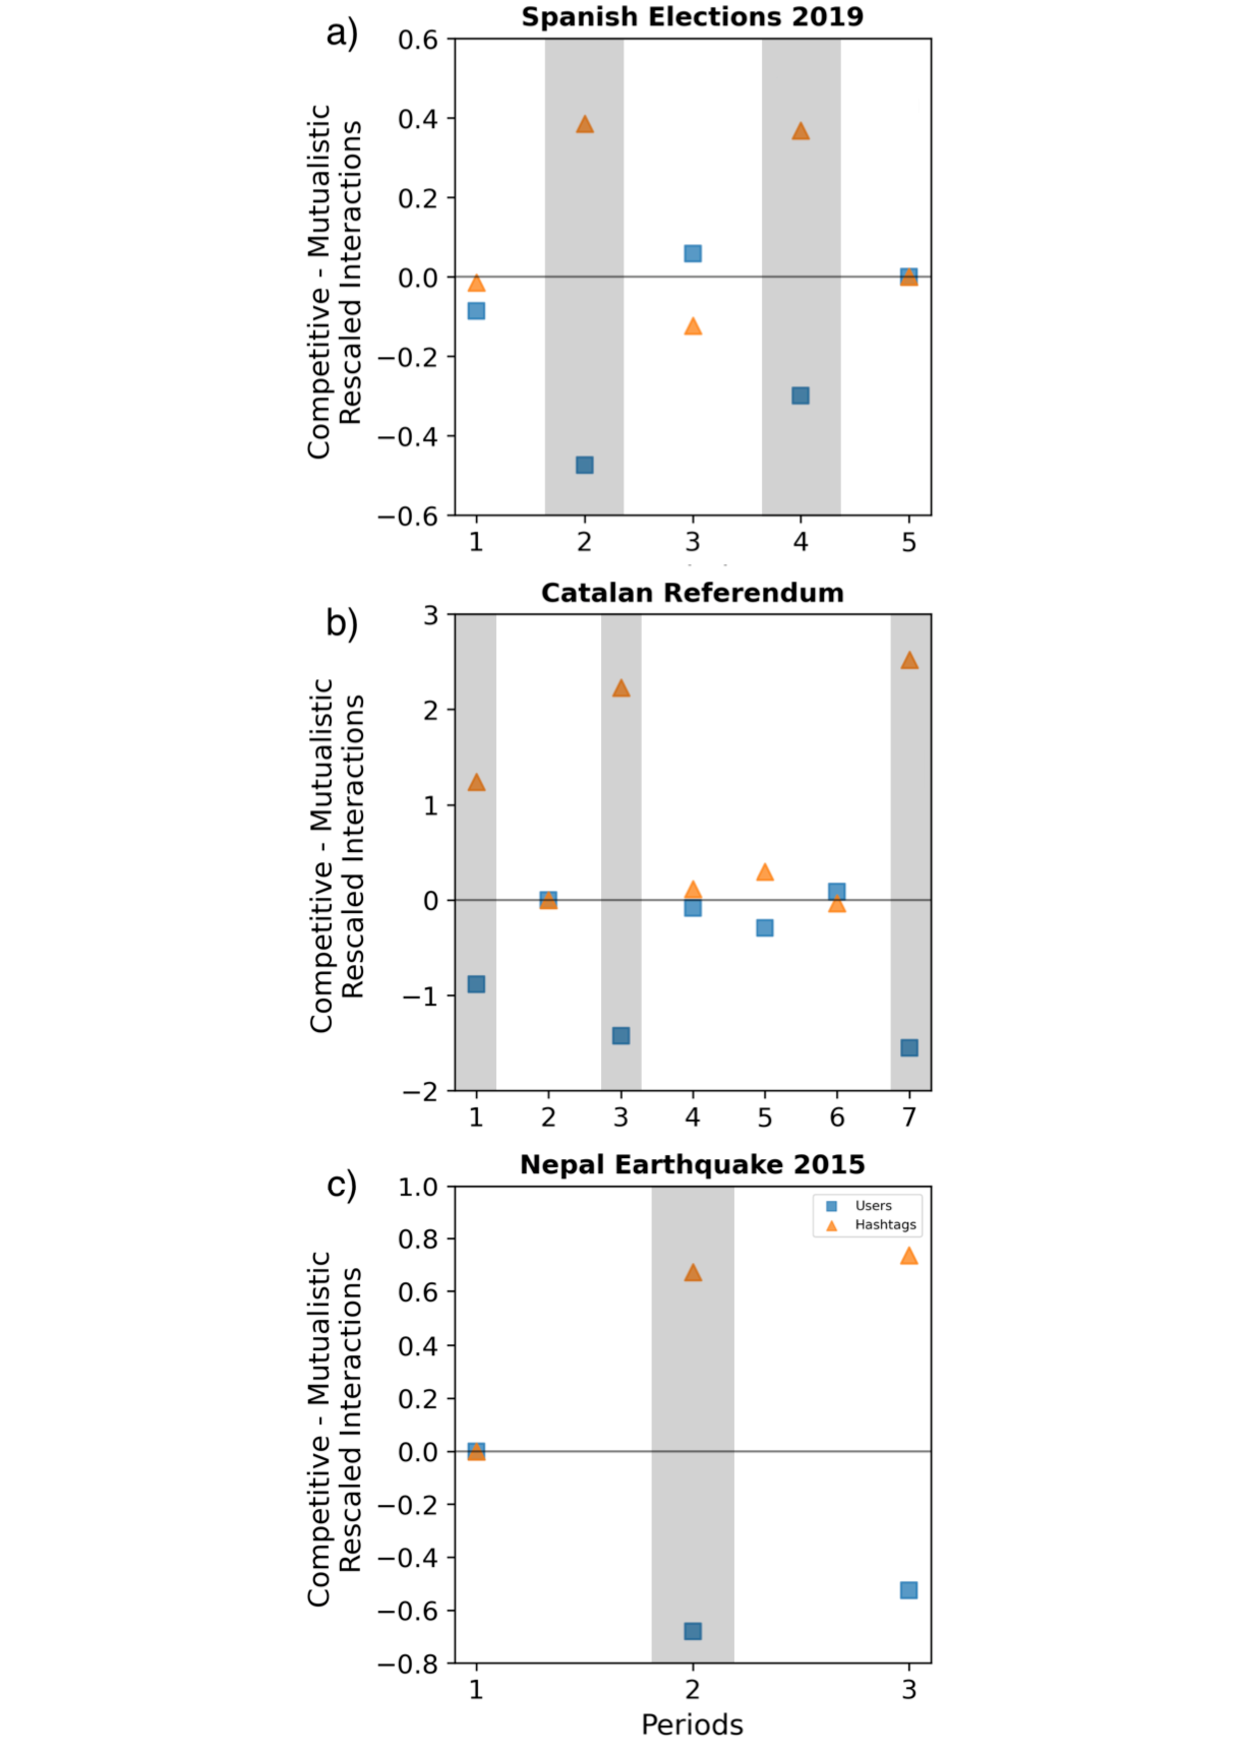
\includegraphics[width=0.5\textwidth]{figures/chp3/fig8.pdf}
   
    \caption[Rescaled difference between competition and mutualism]{Rescaled difference between competition and mutualism over all the periods.  Each point is the average difference between competitive and mutualistic strength for each user (or hashtag). The difference has been rescaled with the values observed during the calmest period (fifth period for the Spanish elections, second period for the Catalan Referendum dataset, and first for the Nepal earthquake). Shaded areas indicate peak periods.}
   \label{chp3:fig:8}
\end{figure}


The results so far in Figures~\ref{chp3:fig:4a} to~\ref{chp3:fig:6} can be easily understood in terms of visibility maximization. In normal times, users tend to focus on their specific interests and aim for visibility inside their communities. Important events can captivate everyone's attention, leading users to join the conversation. This simple response, driven by individuals' strive for visibility, has some complex consequences. On the one side, an increase in competition for attention. With a huge amount of messages covering one single topic, the probability for each user's ideas to be heard decreases. On the other side, the use of hashtags related to relevant topics can lead to a mutualistic (positive) interaction as they allow us to reach a larger audience. Our goal is to quantify the strength of both these interactions to understand which one dominates the dynamics in the different periods.  \\

To achieve this, as explained in Section~\ref{chp3:1.4}, we construct three interaction networks from user and hashtag similarities --two for competition ($\boldsymbol{\beta^{UU}}$ and $\boldsymbol{\beta^{HH}}$), and one for user-hashtag mutualism ($\boldsymbol{\gamma^{UH}}$)-- and examine changes in node strength over time. The benefit of estimating competitive and mutualistic strengths using niche overlap  \cite{cai2021niches} is that it rescales both terms, making them comparable. By doing so, we may calculate how much each factor contributes to the dynamics of the system. \\ \\

\begin{figure}
    \centering
   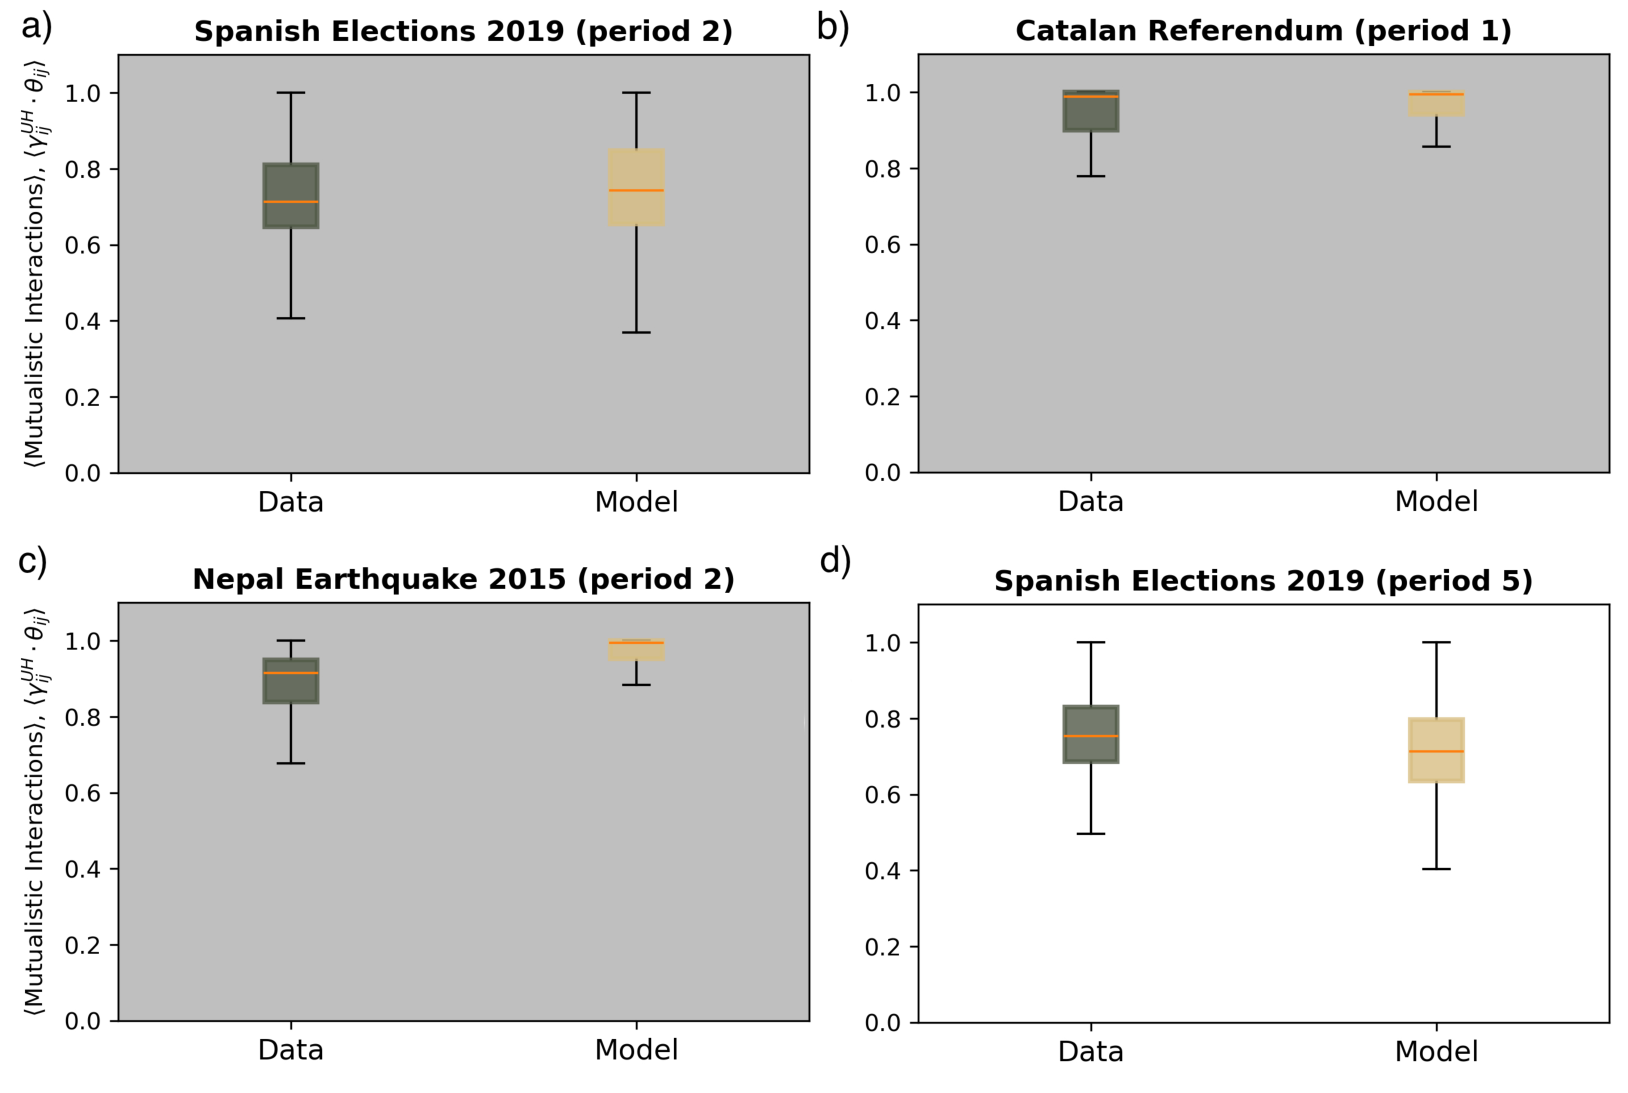
\includegraphics[width=1.05\textwidth]{figures/chp3/fig9.pdf}
   
    \caption[Effective interactions recovered from the visibility optimization model]{The effective mutualistic interaction strengths $\gamma^{UH}_{ik}\theta_{ik}$ extracted from the data (dark brown boxes) to compare with the values obtained with the visibility optimization model (light brown boxes). (Panels a-c) For the calm-to-peak transitions, the model's initial conditions are as follows: 
To emulate an exceptional event, the initial values of matrices $\beta$ and $\gamma$  are the empirical matrices of a high activity period, which correspond to the $400$ most active users together with the hashtags they used from a. In particular, we choose period $1$ for the Catalan referendum and period $2$ for the Spanish elections and the Nepal earthquake. Moreover, the user-hashtag interaction matrix $\theta$, which indicates whether a user posted a specific hashtag, is extracted from the previous or next calmer period. These periods are $1$ for the Spanish elections and the Nepal earthquake, and period $2$  for the Catalan referendum). (Panels d) For the Spanish elections peak-to-calm transition, matrices $\beta$ and $\gamma$  are now selected from a calm period  (period $5$), while matrix $\theta$ is taken from the previous high-activity period (period $4$).  In all the transitions, the model runs for $5 \times 10^4$ rewiring attempts. The rest of the parameters are $\Omega_c = \Omega_m = 0.08$ for Spanish elections and Nepal earthquake datasets, and $\Omega_c = \Omega_m = 0.1$ for the Catalan referendum. The box plots represent the distribution of the values $\gamma^{UH}_{ik}\theta_{ik}$. The orange lines are the median of these distributions, and colored areas delimit the 25th and 75th percentiles.}
   \label{chp3:fig:9}
\end{figure}

Box plots of the interaction strength distributions for the three datasets are displayed in Figure~\ref{chp3:fig:7}. During high-activity periods, we consistently observe an increase in both competition and mutualism. The evolution of the two interactions does, however, differ from one another. Even in times of low activity, users still face competition. Its strength is only marginally increased when an external event occurs and attention shifts as a result. Instead, hashtag competition generally declines during calm periods and increases significantly during events. Similar results are observed for mutualistic interactions, with moderate values (with a median of approximately $0.4$) for resting periods and dramatic jumps up to nearly $1.0$ during peaks. \\

Given the previous results, however, the fundamental question of which mechanism weighs most for users and hashtags remains. To provide an answer, in Figure~\ref{chp3:fig:8}, we show the average difference between competitive and mutualistic strength for each of the $400$ users and related hashtags, rescaled now to the value they had during the calmest period of their corresponding dataset. We notice two distinct behaviors for users and hashtags. As mutualistic strength grows more than competitive strength at peak intervals, the effective competition experienced by users reduces significantly.  Users are encouraged to actively participate in the main debate by this effect since they can see that their posts are getting greater attention. 
Instead, there is typically more hashtag competition during events than there is during other periods. This is likely because hashtags unrelated to significant event topics will receive very little attention, whilst those linked to key topics must withstand the additional pressure brought on by user interests. \\ \\

\subsection{Modeling attention switches during exceptional events}
\label{chp3:2.4}

After evaluating the effective competition that the users faced, we try to identify the key factors that led to the reorganization of the information topics that we observed in the datasets. We use the visibility optimization model described in Section~\ref{chp3:1.3} and \cite{palazzi2021ecological} to do that. While the authors in \cite{palazzi2021ecological} use synthetic data to simulate the model to replicate the structural reorganization of the user-hashtag interaction networks during external events, here we take a step further and use the matrices that have been directly created from the data to inform the model. This will allow us to test the idea that the major cause of the concentration of public attention is visibility optimization and its resulting decrease in perceived competition. \\

In order to demonstrate that visibility optimization is the main driver of the dynamics, we run the model during a transition of two successive periods of our data: a calm period followed by an event --for instance, periods $1$ and $2$ in the dataset for the Spanish elections-- and then, we compare the user-hashtag network optimized at the end of the simulation ($\gamma_{ik}^{UH} \theta_{ik}$) with the one derived from the data.
 (model's parameters are listed in the caption of Figure~\ref{chp3:fig:9}). After that, we confront the optimized effective mutualistic interactions $\gamma^{UH}_{ik}\theta_{ik}$ with the one obtained from the peak period data using the hashtag co-occurrence networks and cosine similarity. Additionally, we examine whether visibility optimization can also explain the transition when users' attention shifts back to their primary areas of interest after the peak has vanished. To do that, we begin the model using matrices $\boldsymbol{\beta^{UU}}$,  $\boldsymbol{\beta^{HH}}$ and $\boldsymbol{\gamma^{UH}}$ from a resting period, and let optimize the matrix $\boldsymbol{\theta}$ from the preceding peak period. \\

In the box plots of Figure~\ref{chp3:fig:9} we compare the matrices from the data and the model for the peak-to-calm transition for the Spanish elections (Figure~\ref{chp3:fig:9}d) and the calm-to-peak transitions for all three datasets (Panels a to c). The fact that there is a consistent agreement between the matrices $\gamma_{ik}^{UH} \theta_{ik}$ in each example means that the optimization method alone can accurately duplicate the intensity of the user-hashtag interaction networks that were derived from the data. This supports our earlier findings, which showed that users who pay attention to hot subjects during external events face less intense competition, and that visibility optimization encourages users to return to their original interests once the event has ended.

\section{The science of hype: discussion}
\label{chp3:3}

The emergence of OSNs (Online Social Networks) altered how our society processes information. We switched from the traditional one-emitter many-receivers model that characterized mass media to a complex network where everyone serves as both a producer and a consumer simultaneously. To prevent information processing distortions like the propagation of false news or the emergence of echo chambers that might skew the democratic discussion, it is crucial to understand the forces that determine our collective behavior in this new environment.\\

In this Chapter, to measure the competition for attention that OSN users face during unusual events and how they react to it, we drew on the similarity between natural and information ecosystems. Specifically, we were able to measure the strength of competitive and mutualistic interactions between users and hashtags using a modeling approach based on ecological niche theory. Our findings demonstrate that, while competition between users and hashtags grows significantly during the event's climax, it is also strongly correlated with a rise in users' mutualism. Interestingly, this turns into a positive gain in terms of interactions for users --who, on average, already face greater levels of competition-- thereby decreasing the net competitiveness. On the other hand, this effect is modest for hashtags, that ultimately experience greater competition. Furthermore, the patterns seem universal since they are independent of the type of event (social, political, or natural) as well as the data-collecting method.\\

Our results shed light on the mechanisms behind the emergence of collective attention in online social media, which has critical consequences for group behavior and information processing. The authors of \cite{palazzi2021ecological} show that external events result in a structural shift in the user-hashtag interaction network by using the same visibility optimization model. Here, by informing the same model with actual data, we are able to explain why this new arrangement is better for users. The fact that the numerical simulations agree with the data indicates that users behave as they do because they want to be seen. Users who participate in online debates tend to increase their visibility within the themes that interest them, creating intense competition inside each topic. The same visibility maximization encourages agents to follow the dominant topic as an event approaches, raising competition but also expanding viewers. This rearrangement of interactions is stable, however, because mutualistic benefits outweigh the more intense competition. \\

Although it is exciting that our modeling has been able to provide insights into users' behavior, it still idealizes the complex dynamics that exist in online social systems. For instance, the assumption that the strengths are the same for competitive and mutualistic interactions $(\Omega_c = \Omega_m)$ is one more simplifying premise in our paradigm. Decreasing the parameter space's size, which is a frequent practice in ecological modeling, is necessary for our framework to properly compare the interaction matrices $\boldsymbol{\beta}$ and $\boldsymbol{\gamma}$. Nevertheless, extracting $\Omega$ from raw data would allow us to answer other questions that require a more accurate description of competitive dynamics in OSNs. \\

Finally, we implicitly presume that competitive (mutualistic) interactions only occur between species of the same (different) guilds, as in the majority of ecological models. However, this approach ignores some second-order processes, such as intra-guild mutualism, which has recently been studied in the literature on ecological modeling \cite{crowley2007,stanton2003}. These effects manifest as beneficial interactions between users or hashtags. For example in Twitter, the increase in exposure a user gets when their tweets are retweeted by another user, or how coexisting  hashtags in the same tweet enable each of them to reach a wider audience. These processes might be included to better understand the dynamics of endogenous Twitter events, the rise of important users, and other phenomena.\\




